\documentclass[a4paper,12pt,twoside]{article}
\usepackage{rhreport}

\begin{document}
\thispagestyle{empty}
\begin{center}
    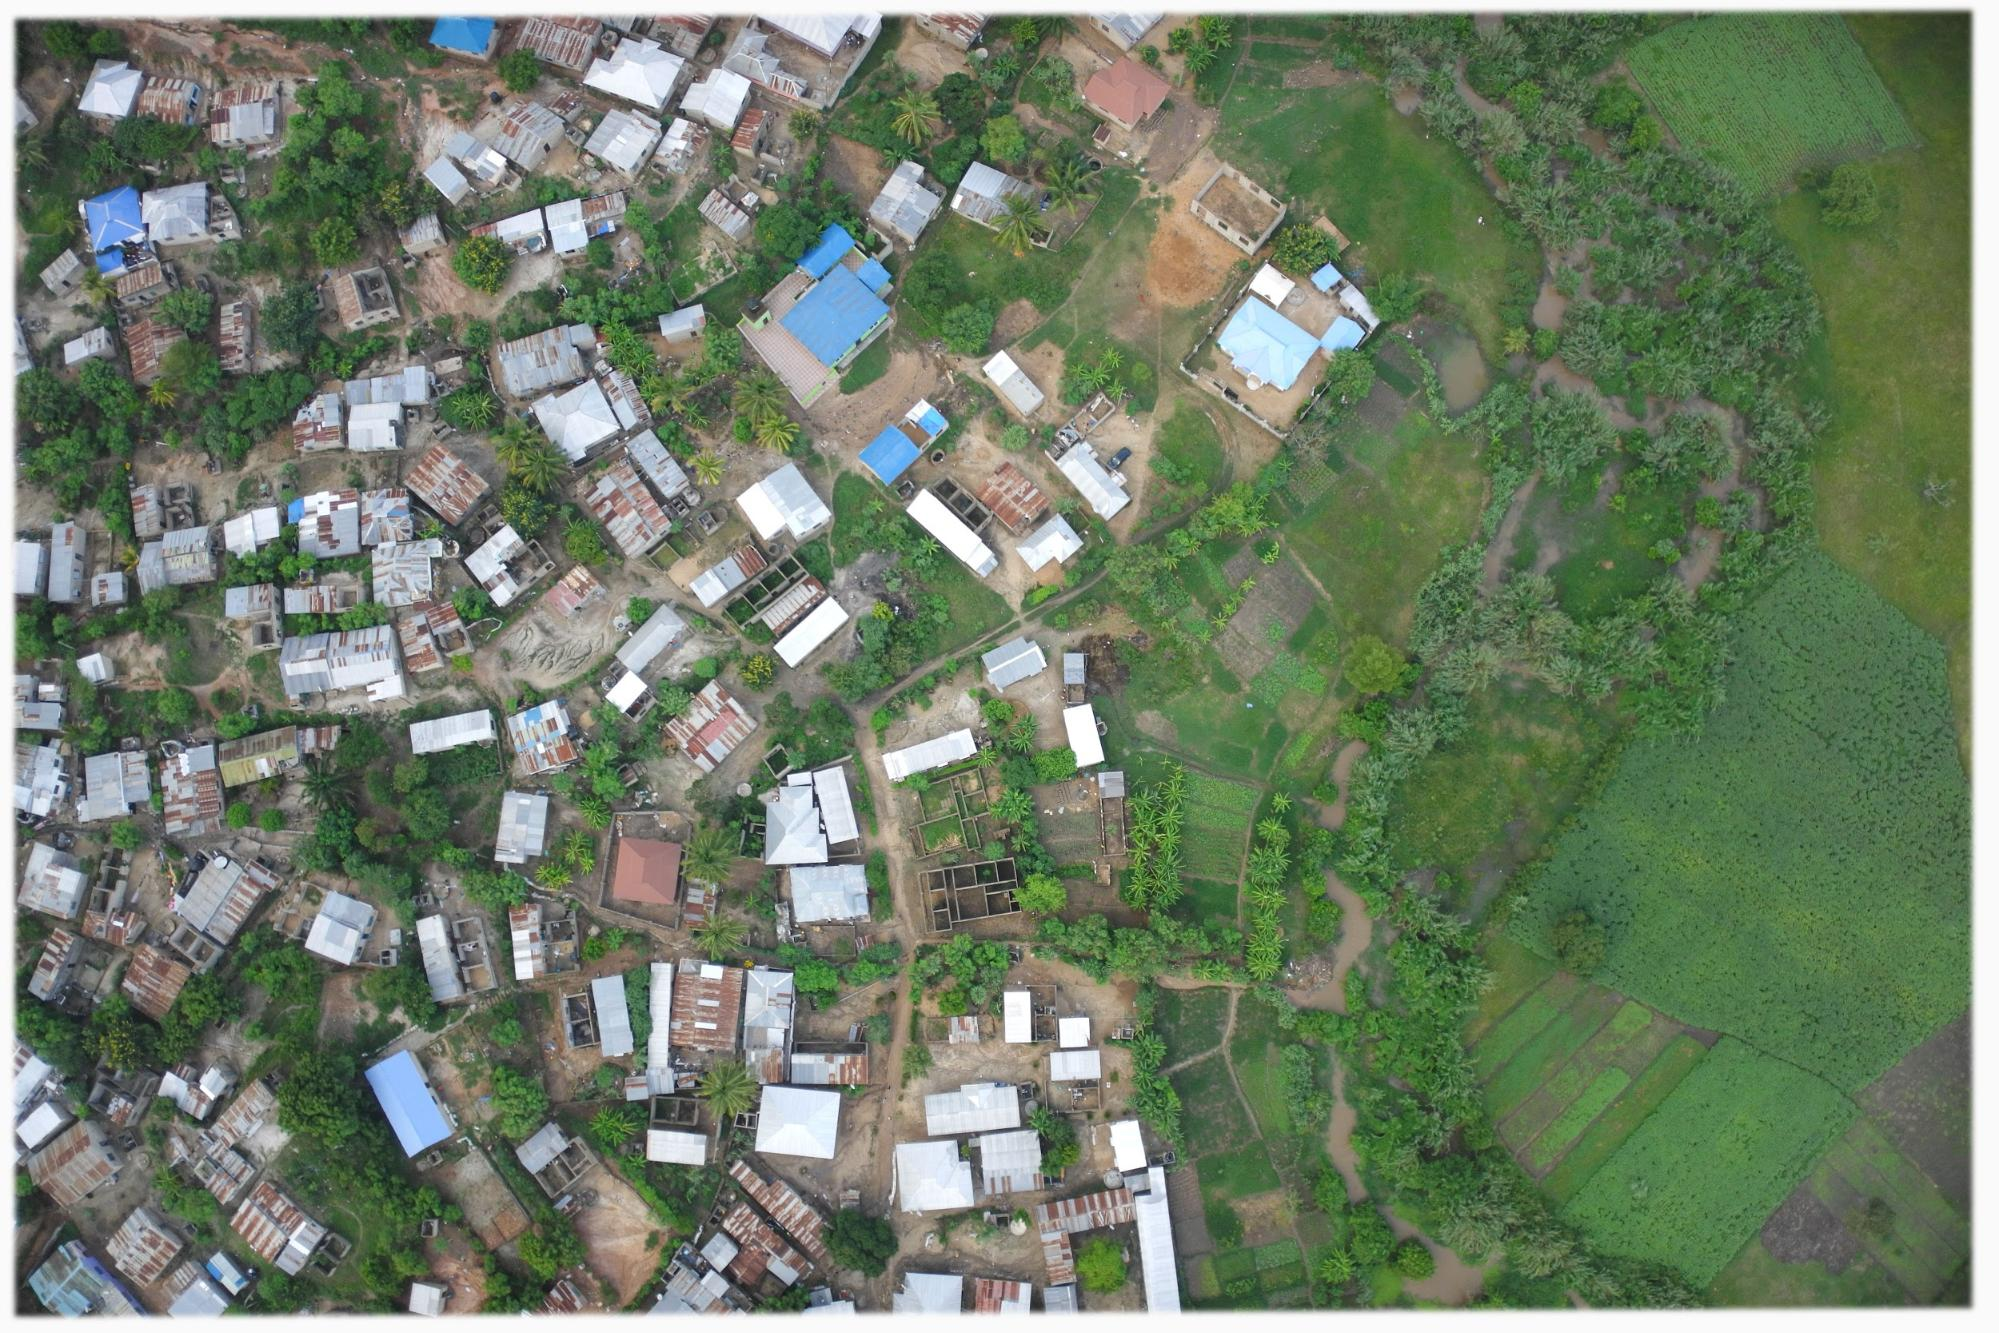
\includegraphics[width=1\textwidth]{images/image1.jpg}
\end{center}

\begin{center}
  \Huge \color{RHblue} \textbf {Aerial Riparian}
\textbf{Solid Waste Mapping}
\end{center}
\medskip

\vbox{
  \centering
  Prepared for:
  \vcenteredhbox{\includegraphics[width=2cm]{}}
  and { }
  \vcenteredhbox{
\includegraphics[width=7cm]{images/World_Bank_Group_logo.png}}
  \
  
  by:
  \vcenteredhbox{
\includegraphics[width=4cm]{HOT_logo_with_text.png}}
  % \maketitle
  
}

%\begin{figure} %[H] 
%   \centering
 %     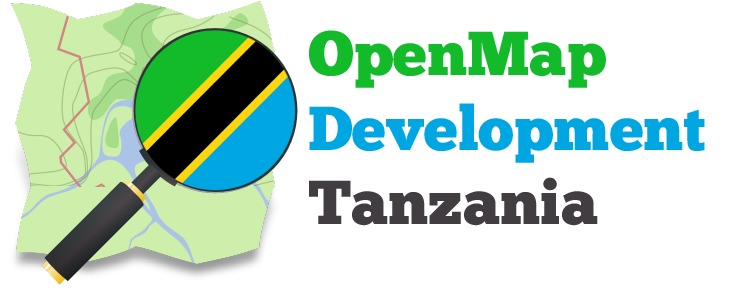
\includegraphics[width=0.3\textwidth]{images/image10.jpg}
%\end{figure}
    
%\title{Aerial Riparian Solid Waste Mapping}
%\author{OpenMap Development Tanzania}


\date{August 2019}


\maketitle

\bigskip \bigskip \bigskip \bigskip \bigskip \bigskip \bigskip \bigskip \bigskip \bigskip
\bigskip \bigskip \bigskip \bigskip \bigskip \bigskip \bigskip \bigskip \bigskip \bigskip \bigskip \bigskip \bigskip \bigskip \bigskip

This report was prepared by Glory Emanuel, Bornlove Ntikha, Iddy Chazua, Dorica Mugusi, Tonny John, Immaculate Mwanja, Aaron Eubank, Hawa Adinani, Innocent Maholi, Ivan Gayton, William Evans


\newpage
\tableofcontents

\newpage
\section{Executive Summary}

    \begin{multicols}{2}
    \lipsum[0-3]
    \end{multicols}

\section{Introduction}

    \lipsum[0-4]
  
    Drone flights enable studying any aggregations of waste/informal dumps that are on the banks of the waterways within fifty metres of its bank on either side.Such data is presented as three-dimensional imagery of waste aggregations, further assisting the study team to estimate rough waste volumes.
    
    Drone flights consistently track and record spatial data relating to their own trips and correspond the GIS data with a set of other socio-political and economic indicators, to ease further analysis. This includes:   
    
    \begin{itemize}
        \item The corresponding political division i.e. subward, ward and municipal boundaries—drone flight spatial data overlaid existing socio-political spatial data indicating, via simple desktop analysis, the political constituency that governs each spatial area the drone covers. This allows users to correspond with an informal/illegal dump with the relevant political office that governs the area.
        \item The corresponding density of the geography they are flown over i.e. buildings per sq km/population per sq km via census data. 
    \end{itemize}
    
    
    OMDTZ  combined drone flights and the existing spatial data to conduct a rapid desktop analysis of planned residential and commercial zoning and transport economics as they relate to solid waste management services.
    
    Specifically, spatial analysis allowed the team to quickly present:
    
    \begin{itemize}
        \item Any building or point on a map within the political boundaries of Dar es Salaam that are defined as planned or unplanned.
        \item The complexity of transport from any building in Dar es Salaam to Pugu Kinyamwezi dump site---accounting for two-axle vehicle access, road surface and type, distance and time. 
    \end{itemize}
        
    Datasets provided audiences with vital data on the inequality of solid waste management infrastructure by geography, as well as providing service providers and government with valuable data on what types of transport modes can be employed to service residents and businesses in planned and unplanned geographies of the city.  
    
    Thereafter, OpenDataKit (ODK) Collect,Kobo Toolbox & QGIS trainings were provided to Nipe Fagio staff. OMDTZ provided an in-depth training on how to upload, analyze and present visual data relating to waste hotpots, informal dumps and cleaning activities.


\newpage
\section{Objectives}

    The broad purpose of this work is to provide Nipe Fagio, I4ID and other partners with high-quality and interactive spatial data to better understand solid waste management and service quality across all five municipalities of Dar es Salaam. The main focus of the activities will be along all of the city’s key five rivers which are Mpiji, Tegeta, Mzinga, Kizinga and Msimbazi rivers. 

       %Glory
        \begin{figure}%[H] % uncomment "[H]" to force the  image to the middle of the page  
            \centering
            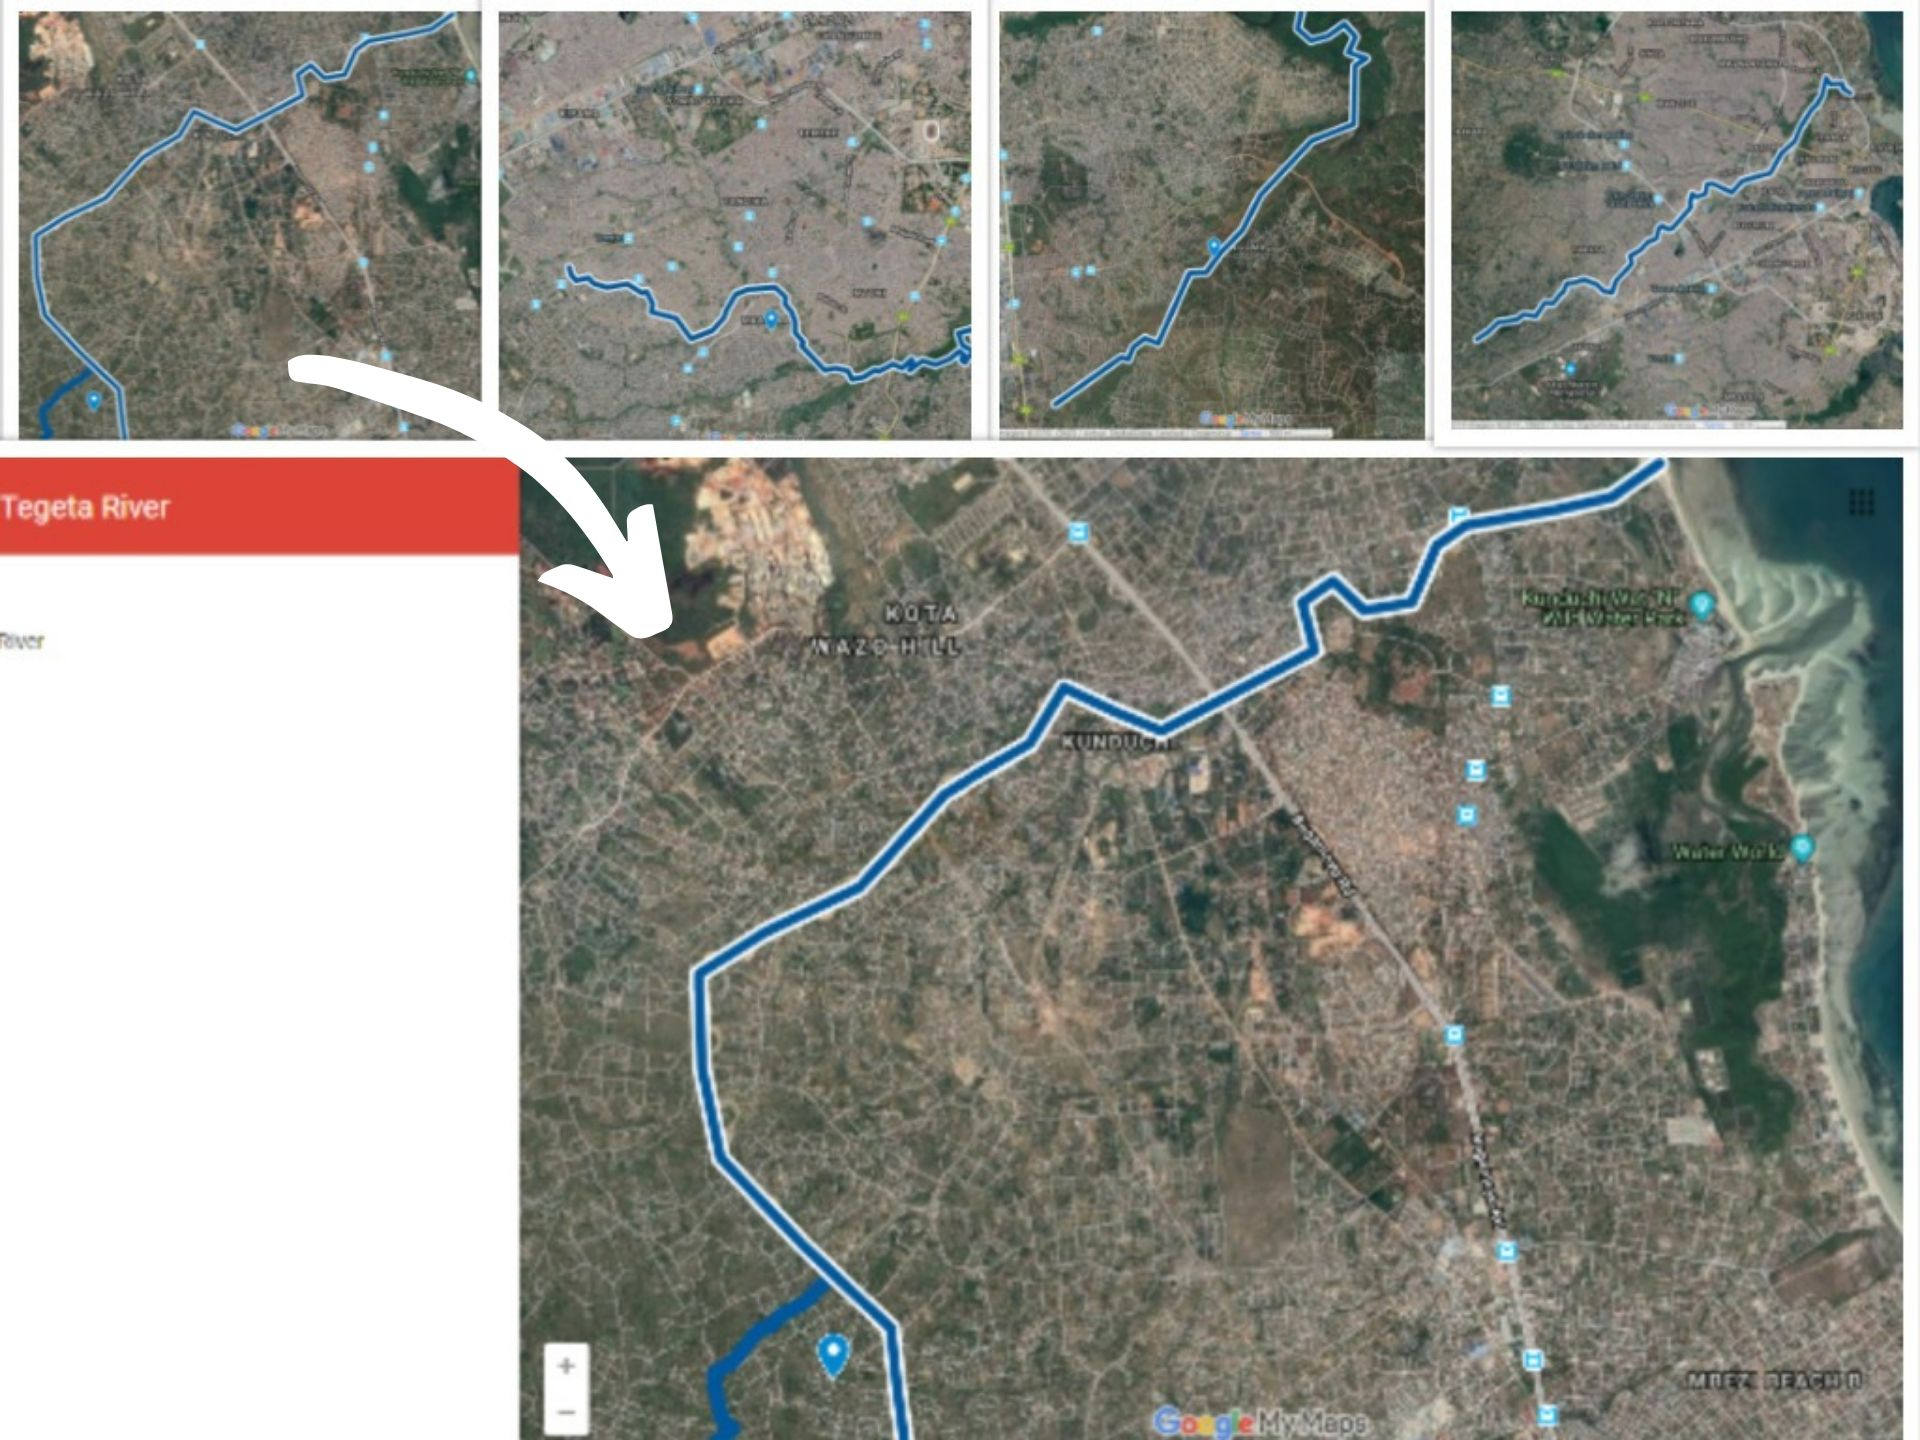
\includegraphics[width=0.8\textwidth]{images/image14.jpg}
            \caption{Screenshot showing missions plans of river mapping}
        \end{figure}

\section{Stakeholders}

\subsection{Implementing Partners}

    \begin{itemize}
        \item \textbf{\href{http://omdtz.or.tz/}{OpenMap Development Tanzania}\footnote{\url{http://omdtz.or.tz/}} (OMDTZ)} %\textbf{} bolds the items
        
        %Bornlove, Glory
        OpenMap Development Tanzania (OMDTZ) is a local registered NGO based in Dar es Salaam and operating across Tanzania. Since its establishment, OMDTZ has promoted a number of community mapping projects, generated map awareness, actively pledged open data sets and continued to build a network of enthusiastic mappers in Tanzania.
    
        \item \textbf{\href{http://uhurulabs.org/}{UhuruLabs}\footnote{\url{http://uhurulabs.org/}}}
    
        UhuruLabs aims to leverage technology and innovation for the development and benefit of Africa and its people. UhuruLabs believes in a world where Africa is an equal and fair beneficiary of its own resources and can take full advantage of technological advancements being made across the world. Projects range from the developing of a multi-rotor drone specifically for use in African agriculture to developing the idea open source toolchain for processing high resolution drone imagery. 
    
        UhuruLabs provided the drones that were used to take the 5cm resolution aerial imagery for mapping four out of five major rivers---Mpiji, Tegeta, Kizinga and Mzinga---in Dar es Salaam city. %aaron
    
    \end{itemize}

\subsection{Beneficiaries}

    \begin{itemize}
        \item \textbf{\href{http://www.nipefagio.co.tz/}{Nipe Fagio}\footnote{\url{http://www.nipefagio.co.tz/}}}
    
        Nipe Fagio, “Give Me the Broom” in Swahili, is a civil society organization founded in 2013. It aims to empower individuals, especially the youth, the civil society, the private sector and government to build lasting change towards turning Tanzania into a clean and sustainable country, conscious through education of its role on waste management and reduction of pollution (air, water, soil).
    
        Nipe Fagio staff were trained by OMDTZ on the use of OpenStreetMap (OSM) local tools for data collection and to use Geographic Information Systems (GIS) to address the issue of waste in the city under their Zero Waste project. QGIS software was executed after the training.

        \item \textbf{\href{https://www.i4idtz.org/}{Institutions for Inclusive Development}\footnote{\url{https://www.i4idtz.org/}} (I4ID)}
    
        I4ID are Tanzanian institutions working to the systems that drive poverty and exclusion. They bring actors together, to design and implement innovative solutions that have the potential for large scale impact.
    
    \end{itemize}

\subsection{Funders}

    \begin{itemize}
        \item \textbf{\href{https://thepalladiumgroup.com/}{The Palladium Group}\footnote{\url{https://thepalladiumgroup.com/}}}
        
        \lipsum[0-1]
    \end{itemize}   

\section{Activity 1: UAV Data Collection}

\subsection{Overview}
    Unmanned Aerial Vehicles (UAV), or drones, were used in this project for collection of high resolution drone imagery to be used for analysis of solid waste dumping sites.
    
    At the outset of this project, drone flights were planned to be  conducted along five major rivers of Dar es Salaam including the Mpiji, Tegeta, Kizinga and Mzinga rivers, spanning 60 linear kilometers of waterways of Dar es Salaam’s critical water arteries. All planned flights were conducted over the course of this project with the exception of the Msimbazi river, where permissions were difficult to obtain due to the proximity of sections of the river to the airport and because high quality drone imagery was generously donated by World Bank. Images from sections of the ________ and the ________ rivers were also generously provided by Tanzania Flying Labs.
    
    Drone flights for data collection were conducted within 44 calendar days from 5th April to 18th May 2019, contingent to the Tanzania Civil Aviation Authority (TCAA) and Ministry of Defence permissions and suitable weather. All technical personnel and equipment required for this assignment are present in Dar es Salaam (site location). 

\subsection{UAV Flights}
    The drone flights provided a digital photographic mark-up of the current status of Dar es Salaam’s waterways. 
    
    Drone flights enable studying any aggregations of waste/informal dumps that are on the banks of the waterways within fifty metres of its bank on either side.Such data is presented as three-dimensional imagery of waste aggregations, further assisting the study team to estimate rough waste volumes.  

    Drone flights consistently track and record spatial data relating to their own trips and correspond the GIS data with a set of other socio-political and economic indicators, to ease further analysis. This includes:
    \begin{itemize}
        \item The corresponding political division i.e. subward, ward and municipal boundaries—drone flight spatial data overlaid existing socio-political spatial data indicating, via simple desktop analysis, the political constituency that governs each spatial area the drone covers. This allows users to correspond with an informal/illegal dump with the relevant political office that governs the area.
        \item The corresponding density of the geography they are flown over i.e. buildings per sq km/population per sq km via census data.
    \end{itemize}  

    Drone flights for data collection were conducted within 44 calendar days from 5th April to 18th May 2019, contingent  to the Tanzania Civil Aviation Authority (TCAA) and Ministry of Defence permissions and suitable weather. All technical personnel and equipment required for this assignment are present in Dar es Salaam (site location).
    
    OMDTZ  combined drone flights and the existing spatial data to conduct a rapid desktop analysis of planned residential and commercial zoning and transport economics as they relate to solid waste management services. 

    Specifically, spatial analysis allowed the team to quickly present:
    \begin{itemize}
    \item Any building or point on a map within the political boundaries of Dar es Salaam that are defined as planned or unplanned.   
    \item The complexity of transport from any building in Dar es Salaam to Pugu Kinyamwezi dumpsite━accounting for two-axle vehicle access, road surface and type, distance and time. 
    \end{itemize} 

    Datasets provided audiences with vital data on the inequality of solid waste management infrastructure by geography, as well as providing service providers and government with valuable data on what types of transport modes can be employed to service residents and businesses in planned and unplanned geographies of the city.

    Thereafter, OpenDataKit (ODK) Collect,Kobo Toolbox & QGIS Trainings were provided to Nipe Fagio staff. OMDTZ provided an in-depth training on how to upload, analyse and present visual data relating to waste hotpots, informal dumps and cleaning activities.

\subsection{Tools}

    During data collection, the following tools were used in site activities:
    \begin{itemize}
  
        \item Spare wings for specific drones (\href{https://www.sensefly.com/solution/ag-360-agricultural-drone/ebee-plus-4/}{ebee plus}\footnote{\url{https://www.sensefly.com/solution/ag-360-agricultural-drone/ebee-plus-4/}})
        \item Spare propellers and rubber to hold the propeller in place
        Umbrella for sunshade used to protect our facilities from rain and sun but also ourselves.
        \item Lithium Polymer (Lipo) batteries and it is bag; enough batteries were packed in the lipo battery bag to help mitigate damage and fire risk to the surrounding objects. Lipo battery bag can save resulting from batteries explosion or fire. Therefore the batteries were packed in the lipo battery bag to ensure safety. 
        \item Radio tracker; this was used to keep track of the drone once it is activated in the drone. This means that you will keep track of the drone, provided that it has this device with it and on, on board you will have Radio Transmitter and on the ground you will have radio receiver in which the radio transmitter will emit radio signals of dedicated frequency in which with your receiver you have to squawk the frequency that will match with that coming from the transmitter on board thus will produce the sound to indicate the matching frequency. How to locate the Drone that has radio Transmitter on it will be simply by using receiver to point on different direction fetching for the where the radio is coming from, once you get the strong signal, you will bet the clean beeping sound from the noise beeping sound, then you will have to move towards the direction where the clean sound is made.
        \item UHU Glue for Polystyrene minor repair
        \item MicroSD cards for swapping
        \item Reflector vest
    \end{itemize}

\subsection{Drone Processes}

    \begin{multicols}{2}
        eBee drones (version Plus and X) were used during the river mapping project to track and record spatial data related to their own trips and corresponding GIS data with a set of other socio-political and economic indicators to ease further analysis. Drone imagery is the output of Unmanned Aerial Vehicle (UAV) carrying a camera to conduct imaging mission. The image is then GeoTagged with Drone Log data that is stitched together to get the output according to the pilot’s desire (Orthomosaic). After the processes explained above, the images were compressed for further use on light processing machines like mobile phones for mapping exercises of trash point location identification.
    \end{multicols}
    
    \subsubsection{Flight Planning}
        This is the process of identifying the area that data collection will be conducted using the UAV i.e. the place where the drone will be flown for aerial imaging. This process is done in the office using base map data from the ground station. Some key notes to consider during flight planning after identifying where the mission will be conducted include: where the takeoff will be set, en route, landing, name of the mission i.e. after creating one, setting up the overlapping━lateral and longitudinal. While abiding with the rules of aviation, you have to set your ceiling drone━top geofencing, setting up the working radius━horizontal geofencing---this is the distance from where your ground station will be located to the end in lateral. Flight planning will be done with reference to the client’s needs but in communication with Civil Aviation Authority or any other responsible board.
    
    \subsubsection{Pre-Flight Checklist}
    
         \begin{figure} %[H] 
            \centering
            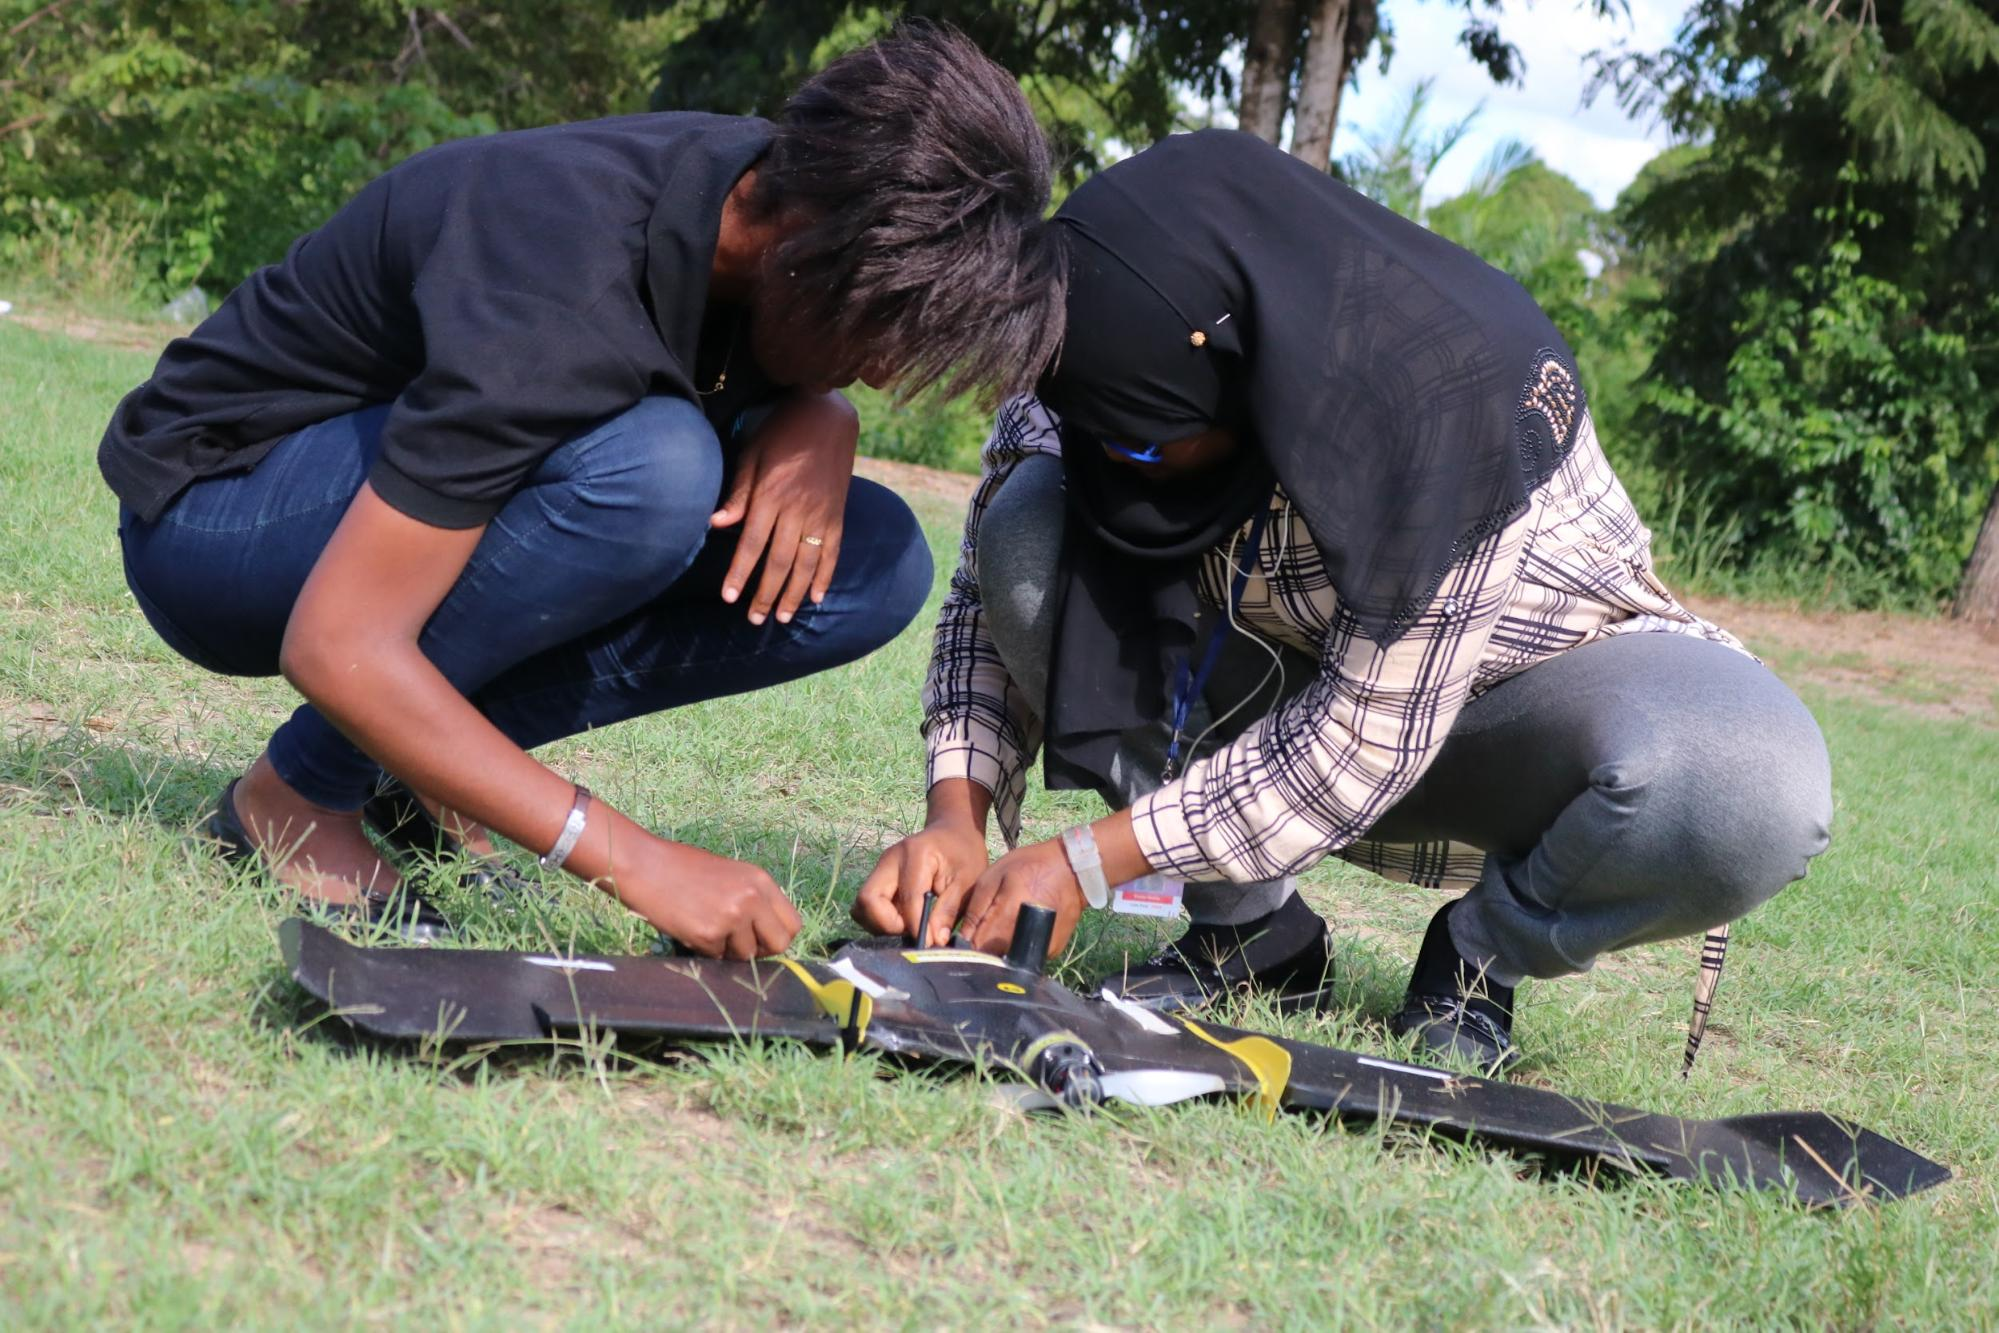
\includegraphics[width=0.8\textwidth]{images/image18.jpg}
            \caption{Pre-Flight check for the ebee plus before take-off}
        \end{figure}
    
        This involved various activities that should be considered prior to the flight in order to make sure everything is ready for the flight to be conducted. This includes aircraft visual inspection, inspecting for controlling parts i.e. if they are working as desired, verifying of planned mission to see the feasibility with the actual area, Takeoff and Landing approach verification, inspecting for SD card status, choose good battery and plug in to the drone, camera function, etc. to make sure drones and other tools are set.
    
    \subsubsection{Take-Off and Landing}
        In this process, the drone was launched for mission to take pictures. When the mission was completed, the drone was commanded to return to its home-way point. The time for the mission to be completed depends on the weather and the power of the battery.
    
        \begin{figure} %[H] 
            \centering
            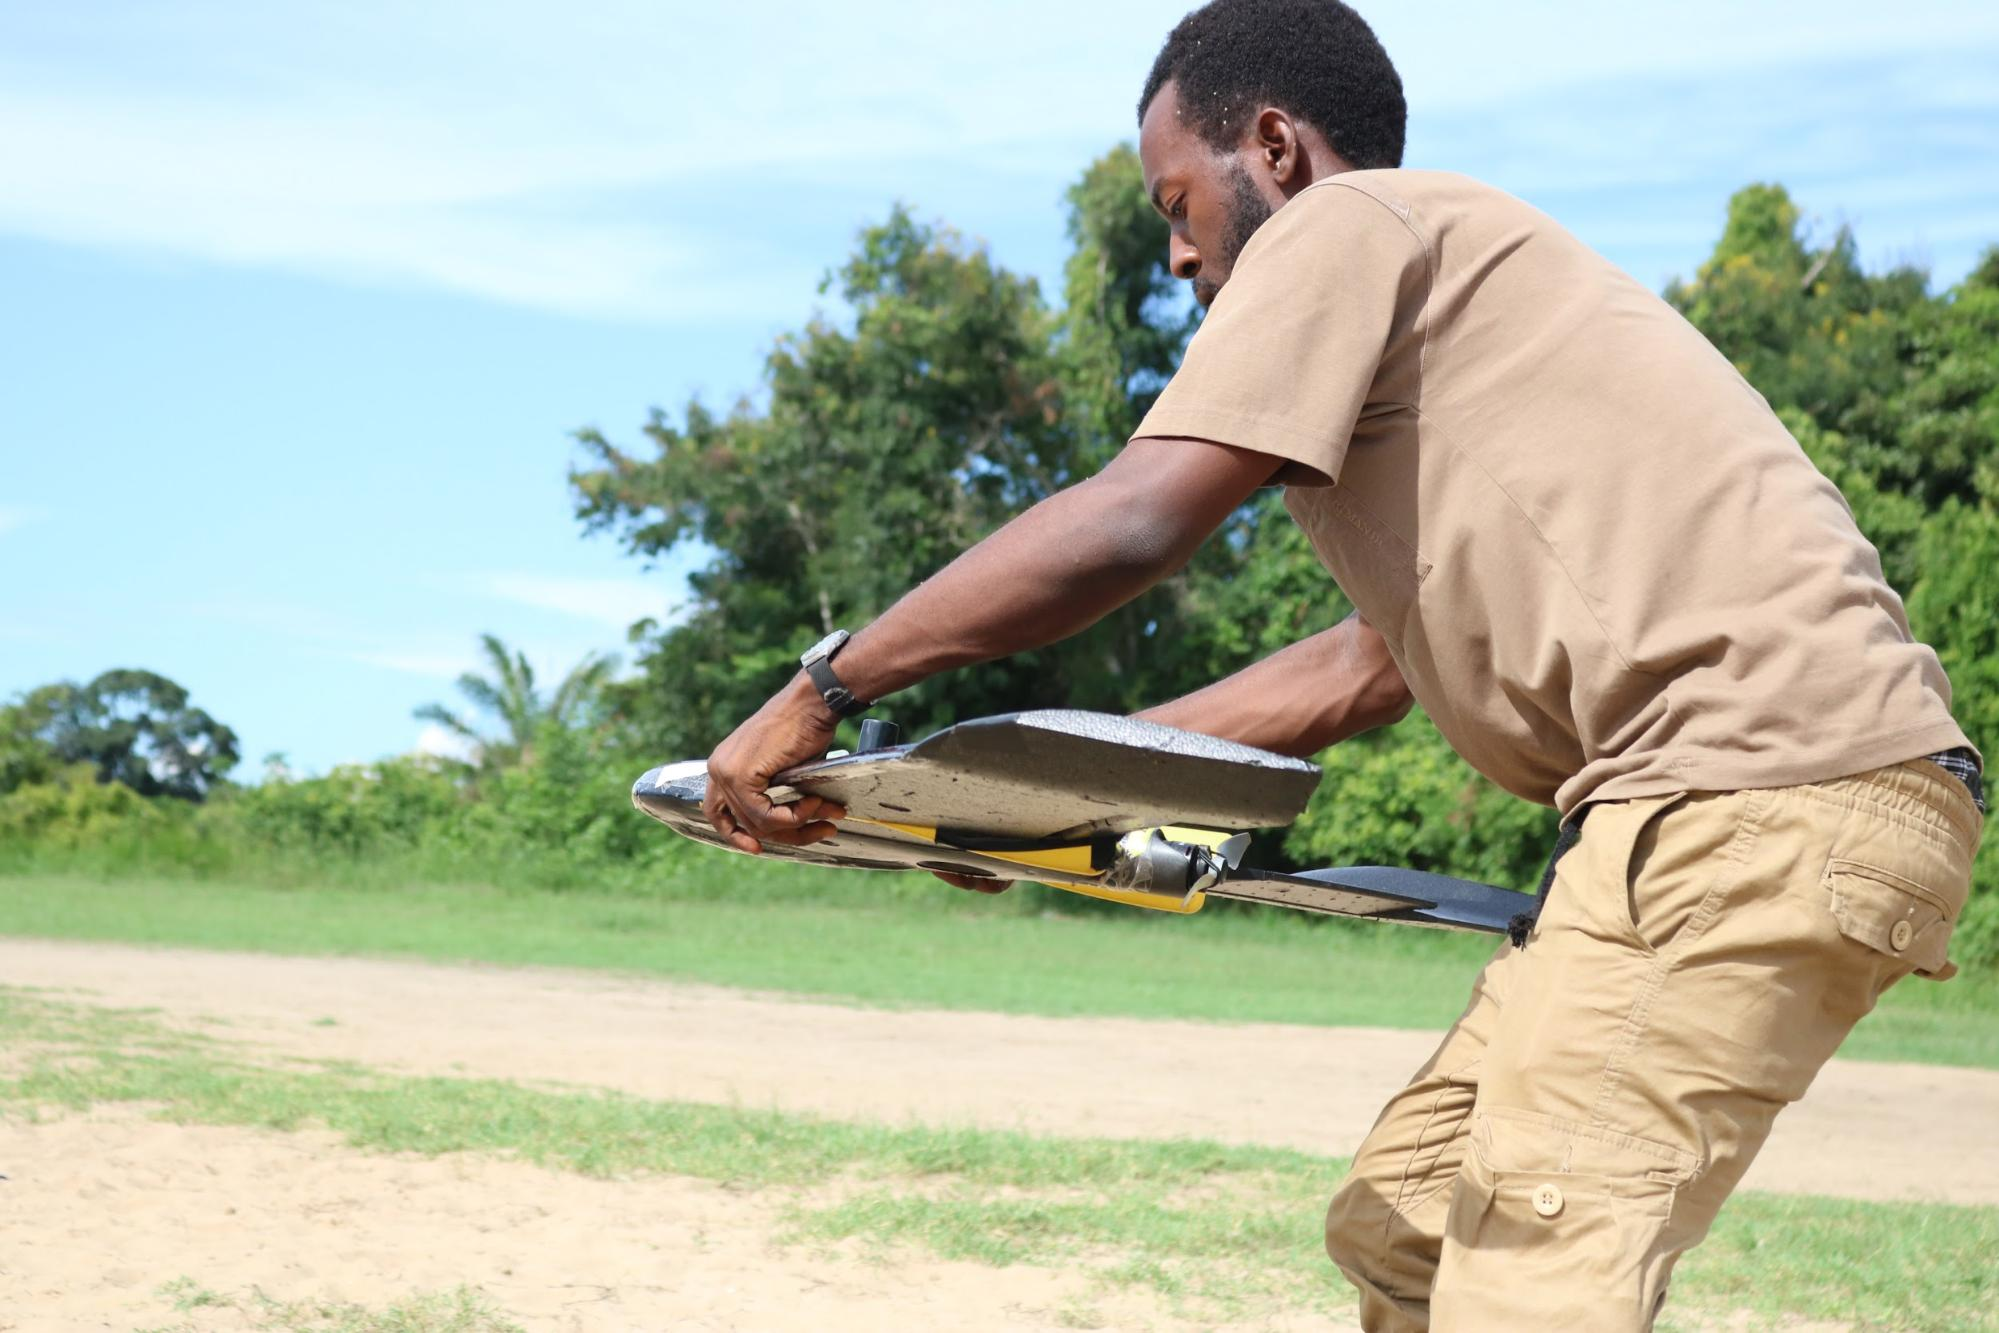
\includegraphics[width=0.8\textwidth]{images/image6.jpg}
            \caption{Launching of ebee plus drone for take-off}
        \end{figure}
    
    \subsubsection{Data Export}
        This process was done after the drone flights whereby images were exported by copying them from the SD card in the drone to the computer. In exporting the BBX, the flight’s log was recorded from the drone and kept in the flight control memory in a computer for post-processing. 
    
    \subsubsection{Data Gathering}
    
    \subsubsection{Data Processing and Analysis}
        After gathering data from the drone and base station, the following had to be done to make the data useful:
        \begin{itemize}
            \item Data from the camera/images were synchronized with drone data (flight logs) using emotion━a program for flight planning and controlling the ebee drone that was used, synchronization of images with flight logs aimed to geo-tag them; this will enable the images to have x-latitudes, y-longitudes and z-elevation information, therefore match with Coordinate Reference System (CRS).
            \item Pix4D software was used to get dataset from single geo-tagged images. The system from the software stitched all the images together and combined them with the data from the GPS base station to increase the accuracy of x, y and z values and came up with orthomosaic data and Digital Surface Model (DSM). The output from the second process will be in regards to what the system has been requested to process and the processing time will vary according to the output needed since they depend on the details needed to provide the desired output.
        \end{itemize}
    
        The generated orthomosaic data will become useful for mbtiles generation to be used for low processing devices like mobile phones. The data is also useful for digitization using JOSM or further analysis with QGIS. DSM is useful for further analysis suitable for waste management alongside rivers as well as analysis of flooded areas near the river banks.
    
\subsection{Results}
    Achievements

    \subsubsection{Target rivers were successfully mapped with the addition of the other six areas.}

        Four out of five rivers i.e. Mpiji, Kizinga, Mzinga and Tegeta rivers were successfully mapped with the addition of other six flight areas---Mpiji small, Ng'ombe, Gama, Base, Kimara A and Kimara B---showing the extent of the trash as shown in the table below:

        \begin{center}
          \begin{tabular}{|c|c|c|c|c|c|}  
            \hline
        	\bfseries AOI & \bfseries Area (SqKm) & \bfseries Total Area & \bfseries Acquisition Status & \bfseries Processing Status\\
        	\hline
            Mpiji Main & 14.357 & 1914 & Complete & Complete\\
            \hline
            Mpiji Small & 4.768 & 644 & Complete & Complete\\
            \hline
            Kizinga & & 2147 & Complete & Complete \\ %Glory, Bornlove
            \hline
            Mzinga & 11.676 & 2019 & Complete & Complete \\
            \hline
            Tegeta & 9.275 & 1306 & Complete & Complete \\
            \hline
            Ng’ombe & & & Complete & Complete \\ %Glory, Bornlove
            \hline
            Gama & 17.389 & 2775 & Complete & Complete \\
            \hline
            Kimara A & 7.574 & 1654 & Complete & Complete \\
            \hline
            Kimara B & 8.8268 & 1707 & Complete & Complete \\
            \hline
          
          \end{tabular}
        \end{center}
        
    \subsubsection{High-Resolution Imagery}
    
        \begin{figure} %[H]
            \centering
            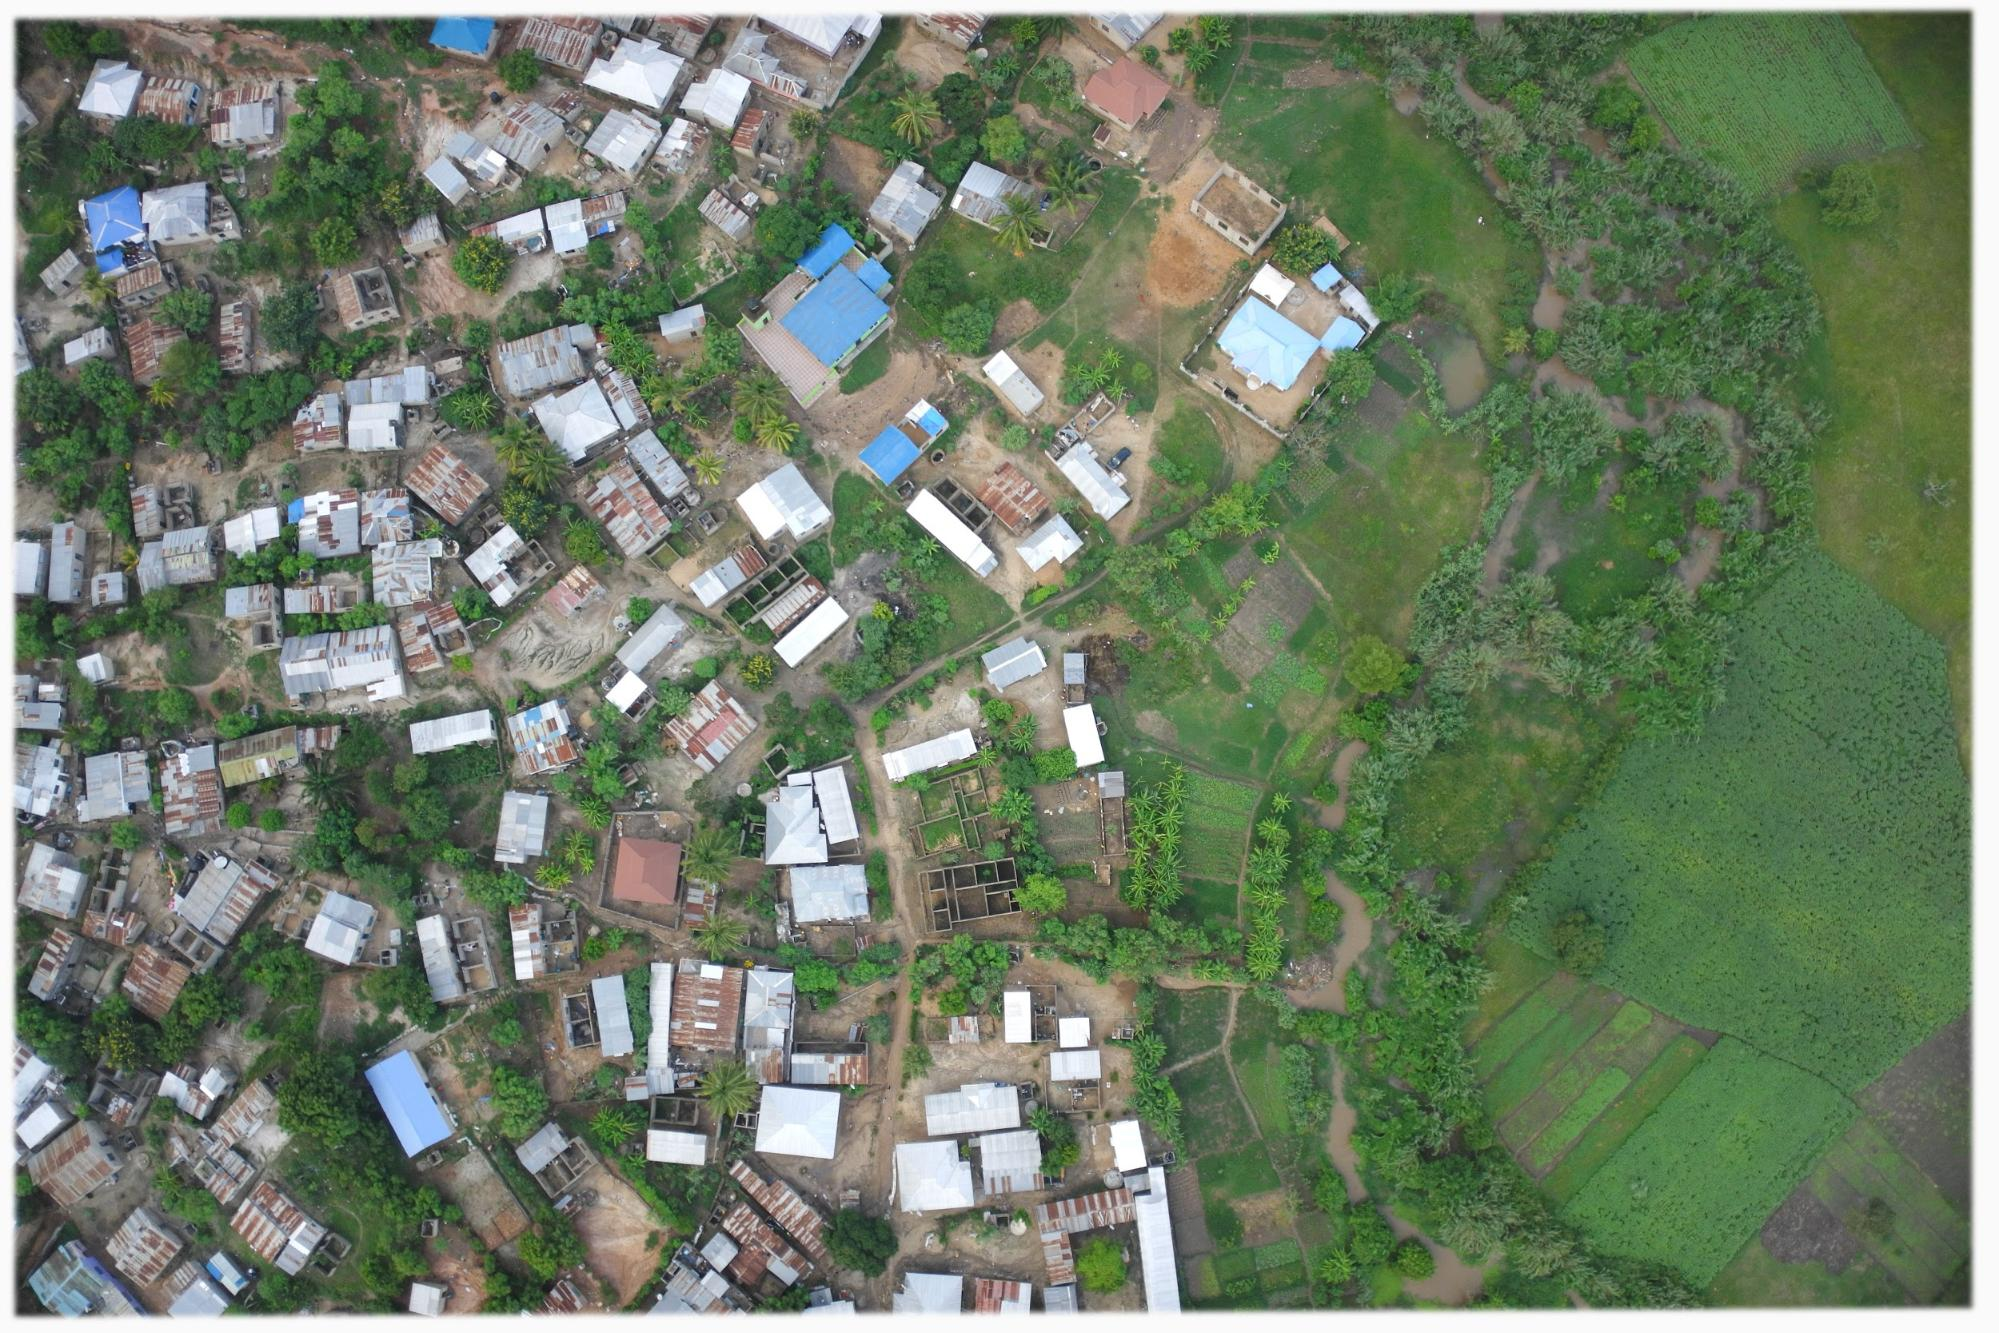
\includegraphics[width=0.8\textwidth]{images/image1.jpg}
            \caption{High-resolution drone imagery showing the location of trash and trash extent along the river and its adjacent areas}
        \end{figure}
        
        The map produced will be from 5cm GSD of high resolution imagery which shows the extent of trash along the river clearly and the adjacent areas that meet the satisfaction of being used in the Nipe Fagio project.
    
    \subsubsection{High-Accuracy Datasets}
    
        For high accurate data set we use Real Time Kinematics (RTK) system. The  drones used were RTK activated and we also employed the use of GPS RTK base station to improve the output being generated regarding x, y, and z values once the data set has been processed.
    
        RTK is the satellite navigation technique used to enhance the precision of position data derived from Global Navigation Satellite System (GNSS) such as GPS, GLONASS, Galileo and BeiDou. RTK uses measurements of radio waves in addition to the information content of the signal and relies on a single reference station of interpolated virtual stations to provide real-time corrections up to a centimeter level of accuracy. With reference to GPS, the system is well known as Carrier Phase Enhancement or CPGPS and is very well applicable in precision land surveying, hydrographic survey and in UAV navigation and surveying.
    
        \begin{figure} %[H] 
            \centering
            \includegraphics[width=0.8\textwidth]{images/image13.png}
            \caption{Real Time Kinematics (RTK) uses satellites and a base station to pinpoint the location of the UAV images with very high accuracy}
        \end{figure}
    
     \subsubsection{Community UAV Awareness and Training}
        Informal education and training on drones were provided to youth from primary and secondary schools, local leaders and community members. Topics included an overview of river mapping, its importance to the development of our community, applicability of drones and river mapping, how to build and operate a drone, its functions and how drone imagery is useful to the community in solving different problems.
     
        \begin{figure} %[H] 
            \centering
            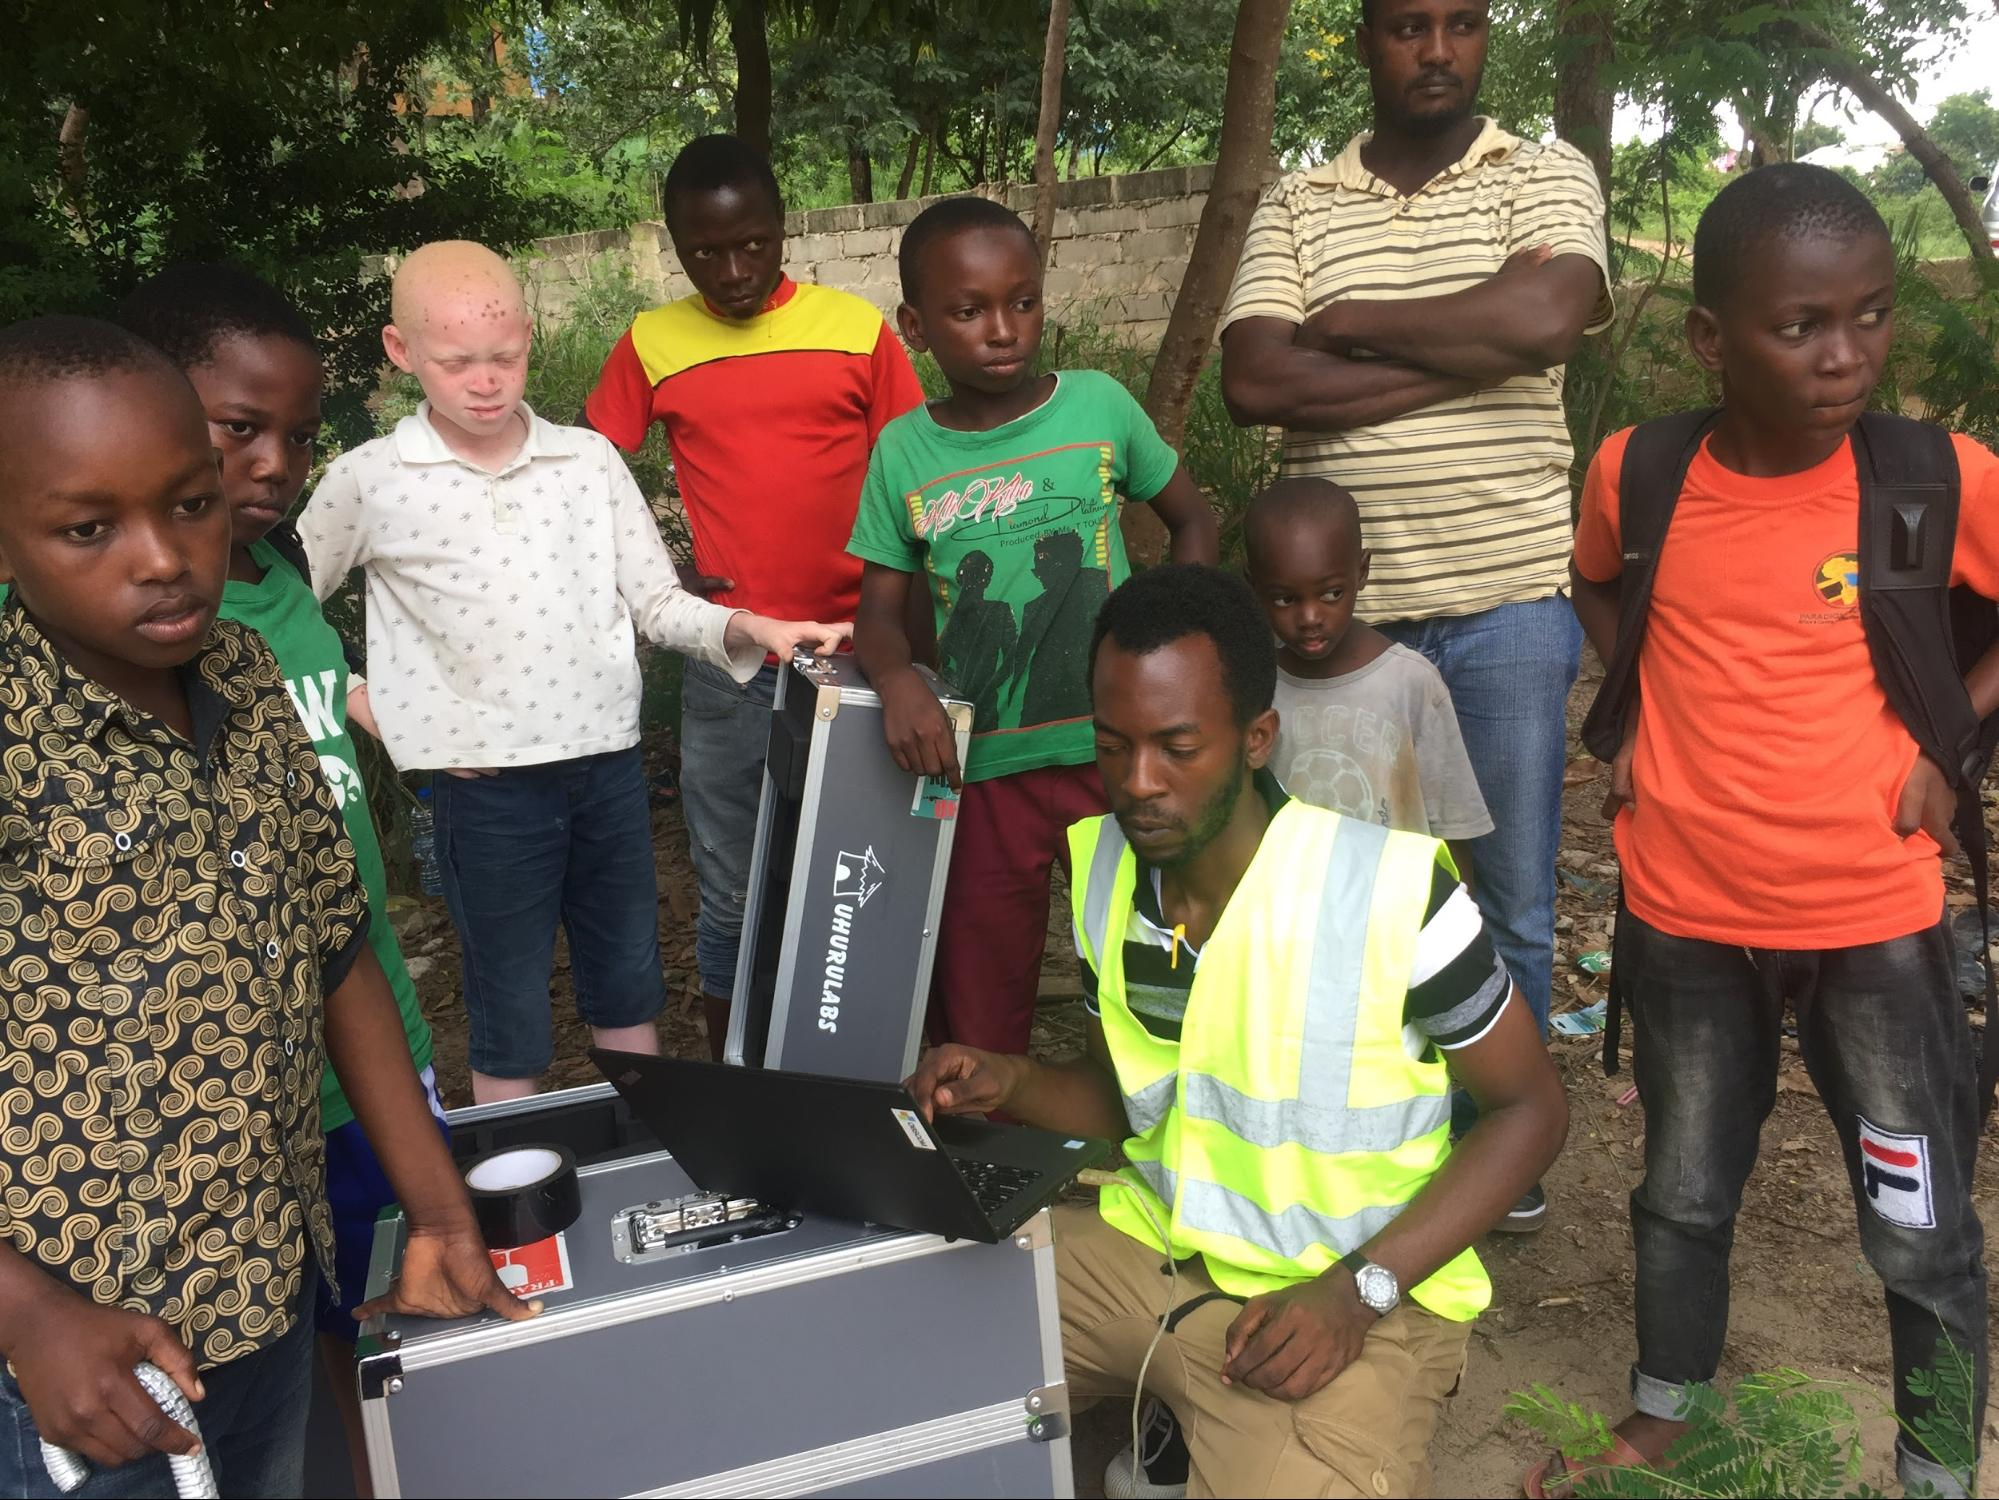
\includegraphics[width=0.4\textwidth]{images/image11.jpg}
            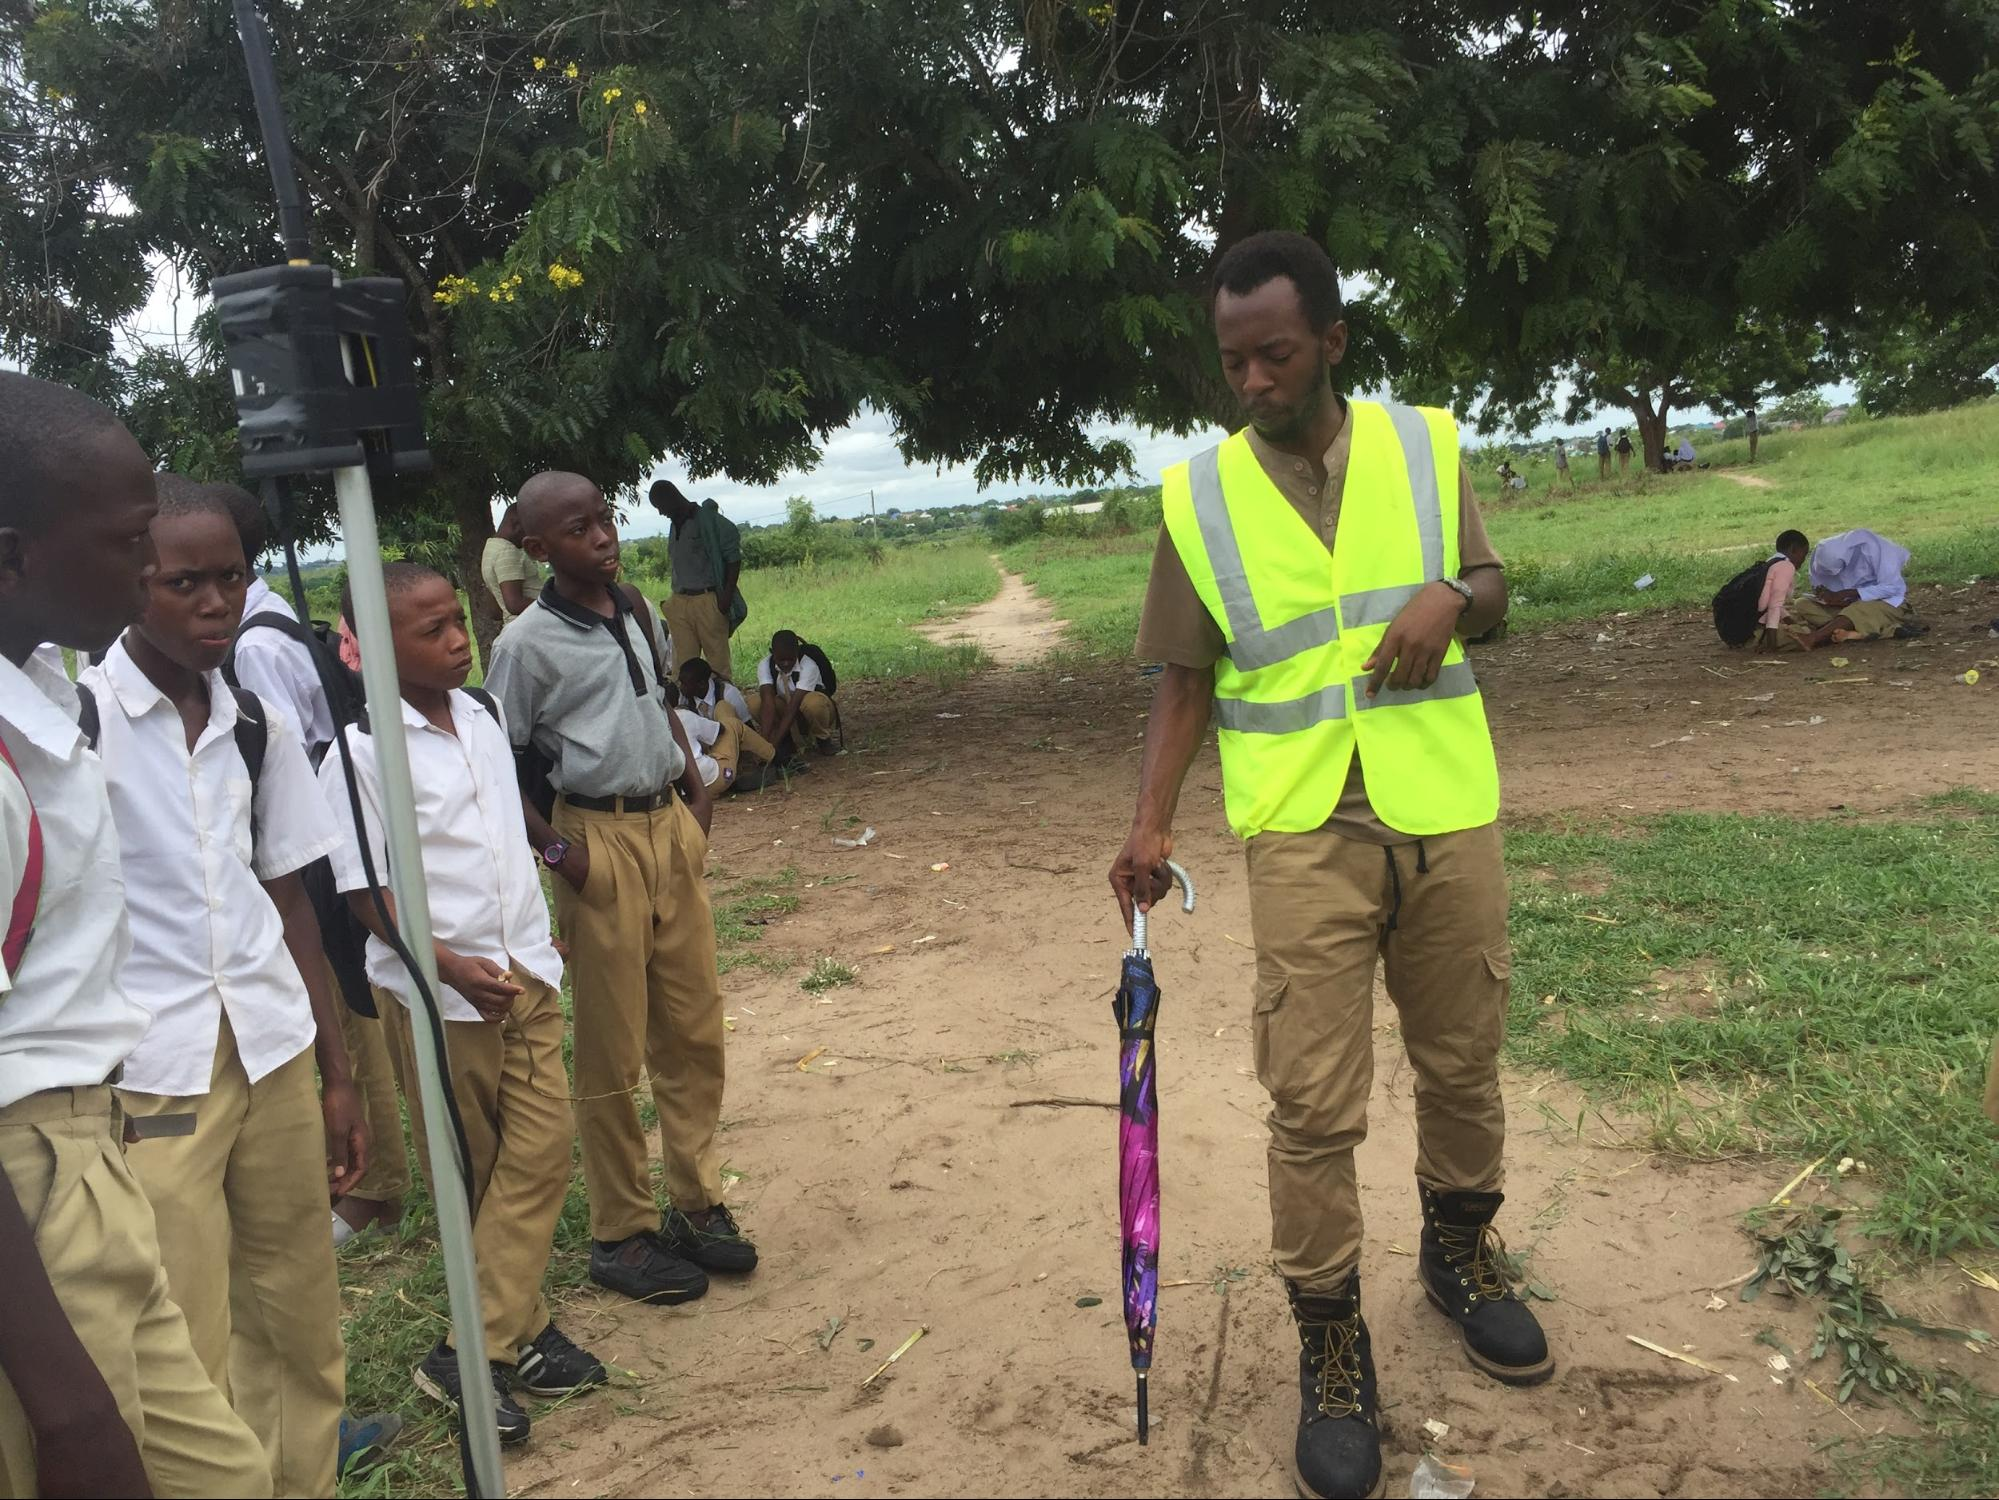
\includegraphics[width=0.4\textwidth]{images/image15.jpg}
            \caption{A group of youth and community members in the field during drone data collection at the Kimara A site}
        \end{figure}
        
\subsection{Challenges: MOVE TO END}
    \subsubsection{Weather}
    
        \begin{figure} %[H] 
            \centering
            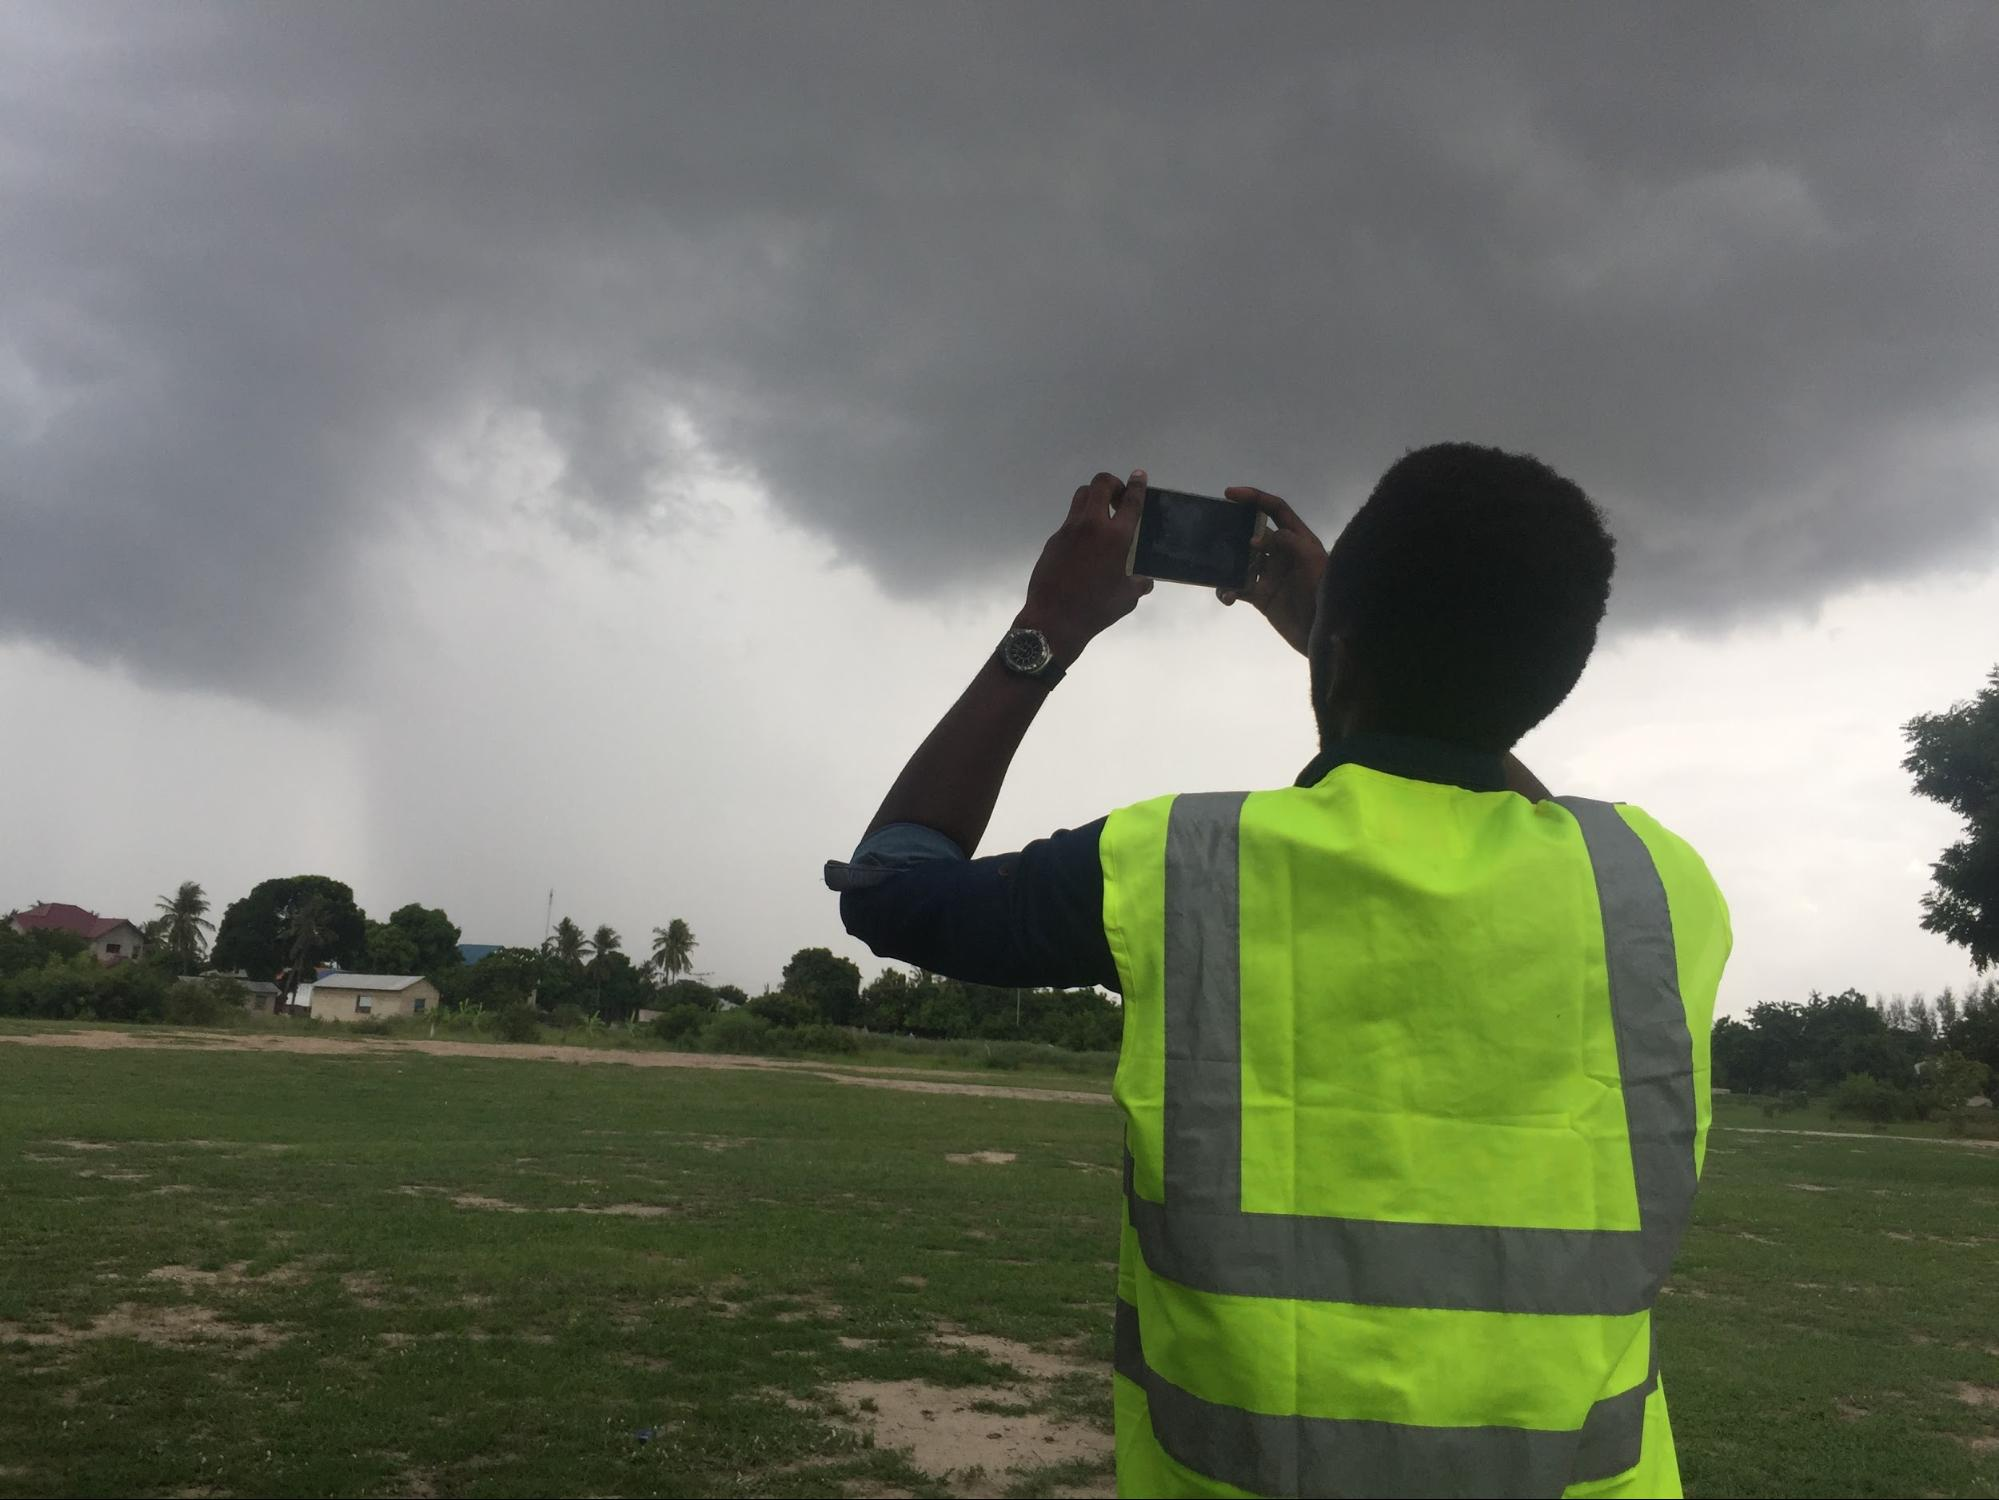
\includegraphics[width=0.8\textwidth]{images/image9.jpg}
            \caption{Sudden storms and inclement weather often interrupted drone flights and data collection}
        \end{figure}
        
        During drone flight in Tegeta river, the weather suddenly changed from a sunny morning to a rainy afternoon. The team had to command the drone to go back to the home-way point of landing in order to avoid crashing of the drone since the battery was highly drained in fighting against the heavy wind and rainfall.
    
    \subsubsection{Permit Delays}
        Getting permits should be the frist step taken in preparation for the flight. In order to conduct drone flights, you need to acquire a permit to operate your vehicle while abiding with the laws governing aviation as well as the underlined government regulations.  Granting flight approval from respective authorities is time-consuming since the approval for operation must go through the Ministry of Defence and the Tanzania Civil Aviation Authority (TCAA) and Intelligent Security Service (ISS).
     
     \subsubsection{Inadequate Take-Off and Landing Areas Onsite}
         Drone flights need enough area for taking off and landing i.e. areas with no obstacles such as trees, power lines, communication towers, etc. The team used satellite images prior to the flights to determine which fields to be used that are closer to mission blocks and suitable for landing. If the field that was identified is not suitable, the team would shift to another field provided that it is close to the mission block as well. The main challenge that the team faced was unsuitability of fields for landing the drones.
     
\subsection{Lessons Learned: MOVE TO END}
    In order to minimize the cost of finding a suitable field, it is important to identify areas prior to visiting them and meeting some criteria for the type of flight that is going to be conducted using tags such as field size, surface area of the field, proximity of obstacles, and UAV aerodrone suitability for conventional Takeoff and Landing or Vertical Takeoff and Landing.
    
\section{Activity 2: Remote Data Creation}

\subsection{Overview}
    The broad purpose of this work was to provide Nipe Fagio, I4ID and other partners with high-quality and interactive spatial data to better understand solid waste management and service quality across all five municipalities of Dar es Salaam main focus of the activities will be done along all of the city’s key five rivers which are Mpiji river, Tegeta river, Mzinga river, Kizinga river and Msimbazi river.

\subsection{Methodology}
    After the acquisition of high-resolution imagery with a 5cm resolution identification of trash piles followed:
    
        \begin{enumerate}
            \item First of all our GIS leads Dorica and Iddy played with imagery on QGIS software to find out what was the common types of waste. They came up with different types of waste such as "plastic_hard", "plastic_soft", household metal, tyres and mixed as well.
            Adding to that they found out the trash points were located near the rivers, in the rivers, along the rivers and others were located within the residences as well.
            \item The second task was the creation of a vector layer(geopackage format) called trash data of which all traced trash polygons with their information were added to it. 
            \item Three mappers with GIS knowledge were then assigned to identify where the trash points are and digitizing them. Apart from that, they identified type of waste and where the trash points located.
        \end{enumerate}
    
    When creating the vector layer for digitization, two main fields were considered when analyzing the imagery:
    
         \begin{enumerate}
            \item \textbf Type of Waste
            After a team member identified a solid waste pile from the imagery she/he tagged which type of waste was found and updated the vector layer. As mentioned above under this kind of field there were these attributes ("mixed", "plastic_hard", "plastic_soft", "metal", "tyres")
            
                \begin{figure} %[H] 
                    \centering
                    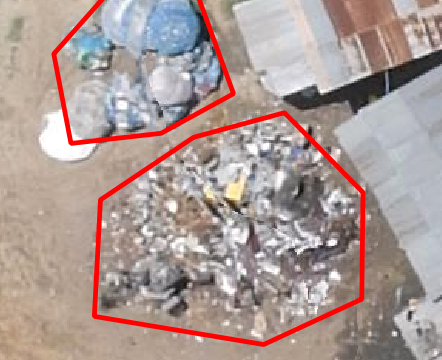
\includegraphics[width=0.4\textwidth]{images/image19.png}
                    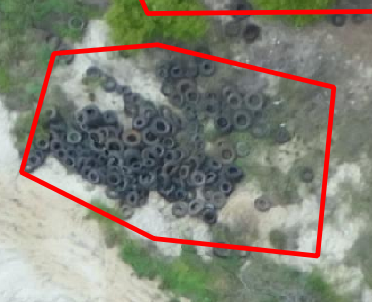
\includegraphics[width=0.4\textwidth]{images/image3.png}
                    \caption{Type of waste = “plastic_hard”}
                    \caption{Type of Waste = "tyre"}
                \end{figure}
                
            \item \textbf Location of Waste
            This field was created so as to tag where the trash points are located. Again ("within residence", "near the river", "along the river" and "in the river") were the attributes under this field.
                
               \begin{figure} %[H] 
                    \centering
                    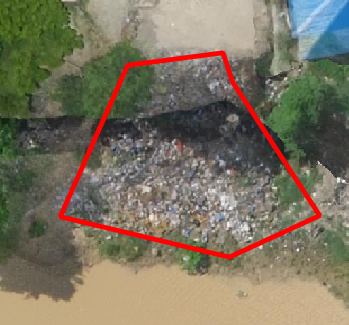
\includegraphics[width=0.4\textwidth]{images/image17.png}
                    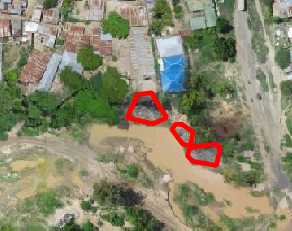
\includegraphics[width=0.4\textwidth]{images/image7.png}
                    \caption{Location of waste = "near the river"}
                \end{figure}
                
                \begin{figure} %[H] 
                    \centering
                    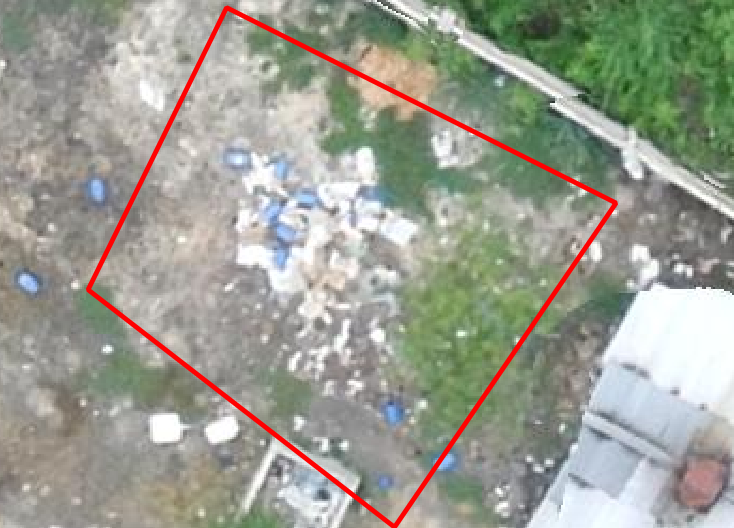
\includegraphics[width=0.4\textwidth]{images/image2.png}
                    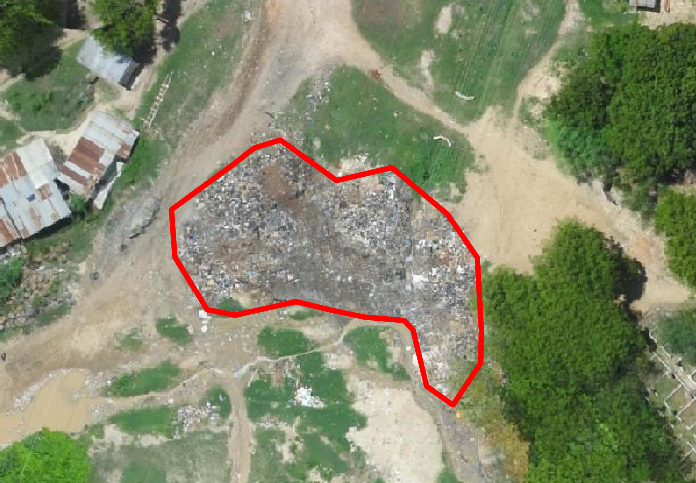
\includegraphics[width=0.4\textwidth]{images/image12.png}
                    \caption{Location of waste = "in river"}
                    \caption{Location of waste = "in residence"}
                \end{figure}
                
        \end{enumerate}
        
         
        
\subsection{Output & Quality Assurance}

    Based on provided drone imageries we were able to identify 1000 trash points.  To achieve the good quality of data Dorica one of our tech people reviewed the data on the attribute table and she found out of 1000 trash points 8 trash points had no information. And finally, 8 trash points were assigned to one of the mappers and got fixed.
    
\subsection{Pilot Ground Truthing}

    This was conducted in Saranga, Kimara and Mavurunza wards by following different procedures:
    
    ODK forms creation

    Mbtiles creation


    2 experienced mappers were sent on the field for data collection activities.

    Since the mappers had OMK and ODK applications on their phones  and knowledge as well they downloaded the survey from the server and got ready for data collection. The mapping supervisor provided them with the drone imagery(in mbtiles format) so as they can identify the trash points in the field easily.

    After collecting imagery and getting the forms they went to Kimara A and B subwards where Kizinga river is to survey the trash points.

    After collecting the information on trash points they pushed the data directly to the server. 
    
\subsection{Results}

    107 trash points were visited and collecting information from them. 4 trash points were not accessible and 20 points were on the imagery but not found on the ground.

\section{Activity 3: Training of Nipe Fagio Personnel}

\subsection{Overview}

    \begin{multicols}{2}
    Dar es Salaam is one among the most rapidly urbanizing cities in Africa with the population in urban areas growing from time to time. There is no question that for some countries or cities, urbanization brings improved access to services and employment, but rapid urbanization poses real challenges for waste management and public health.
    
    Challenges are faced when it comes to the availability and accessibility of geospatial data in the field of proper waste management in the city. To address these challenges, OpenMap Development Tanzania (OMDTZ) in collaboration with Nipe Fagio, carried out a collaborative geospatial training for two weeks. 
    
    During the preparation of launching the Zero Waste project, areas to be surveyed were identified and training on how to collect data using OpenDataKit (ODK) Collect and cleaning the data using QGIS and Kobo server was given to 16 enumerators and 7 Nipe Fagio staff. 
    \end{multicols}

\subsection{Objectives}
    The general objective of the training was to facilitate Nipe Fagio staff on the use of OpenStreetMap (OSM) local tools for data collection and to use Geographical Information System (GIS) to address the issue of waste in the city under the Zero Waste project using QGIS software which was executed after the training.
    
    The following were specific objectives of the training:
        
        \begin{enumerate} %johannes %tonny
            \item Building the capacity of Nipe Fagio staff and enumerators on the OSM tools for data collection.
            \item Creation of Kobo server for aggregating data
            \item Development of household questionnaires for Zero Waste project
            \item Preparation of data collection tools, for example mbtiles, ODK and OSM Tracker 
            \item Reading and preparation of flood-prone (Ramani Huria) maps and base maps for the Zero Waste project
            \item Preparation of Building randomizing and QGIS manual
            \item Field data collection Trash mapping and Validation (People win river win)
            \item Data cleaning with OpenRefine/excel and QGIS
            \item Preparation of a Umap for data visualization
        \end{enumerate}


\subsection{OpenDataKit (ODK) Collect Training}
    
    \begin{figure} %[H] 
        \centering
        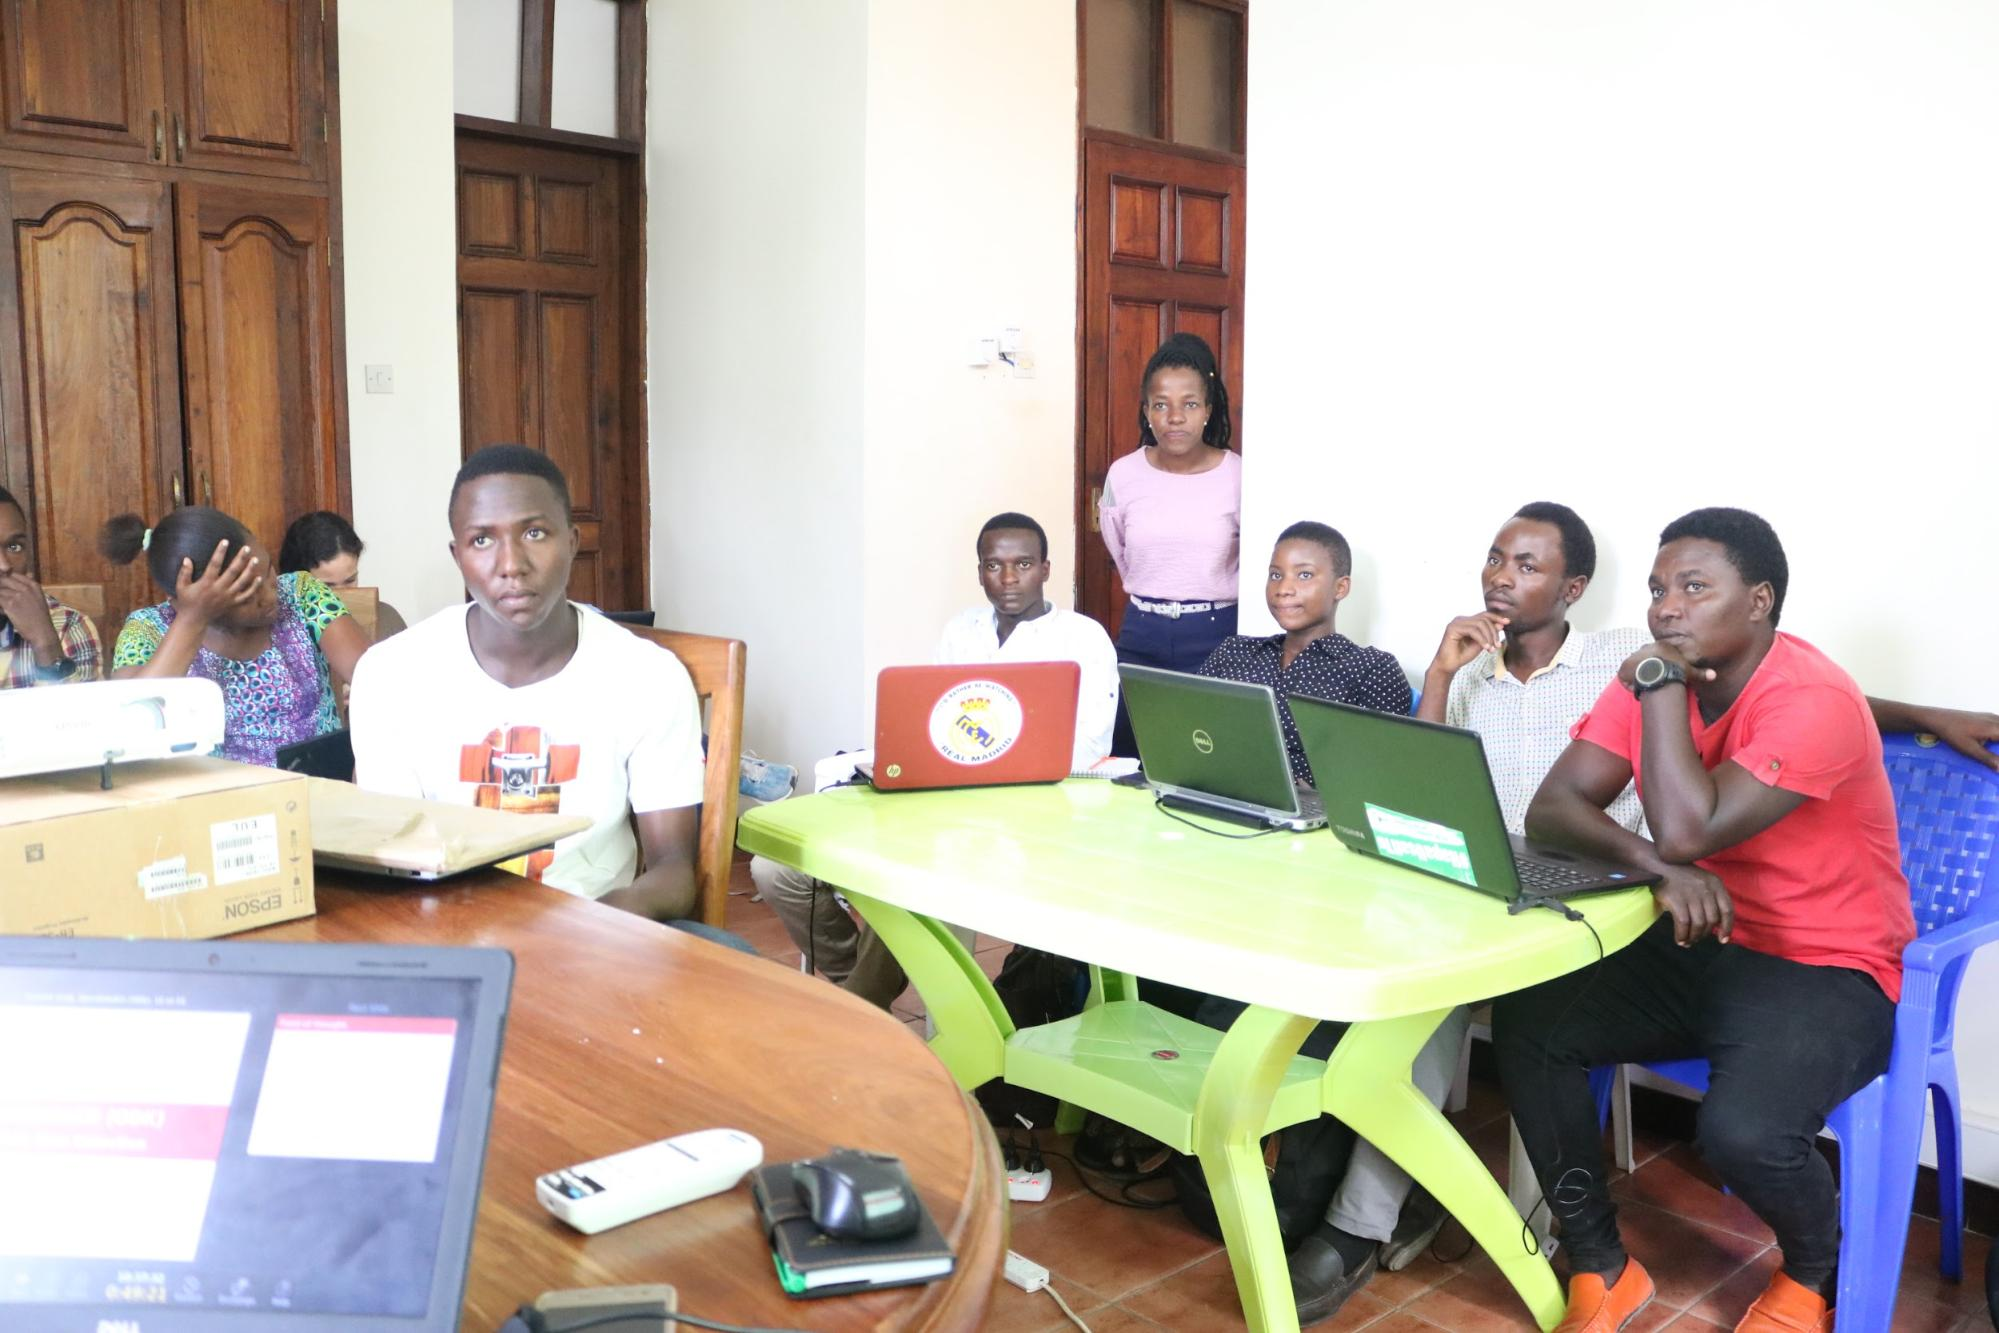
\includegraphics[width=0.8\textwidth]{images/image4.jpg}
        \caption{Nipe Fagio Training at OMDTZ office}
    \end{figure}
    
    ODK training based on how to collect information using the mobile application and how to configure/connect it with the Kobo server. The training also covered how enumerators and community members can work together during data collection. It was important for the enumerators to work with the community members which would facilitate them to create their own maps and would concur with OMDTZ’s motto where community members should create their own maps. 
    
    Before data collection, enumerators were trained for two days on the tools that would be used for preparation for and data collection. On the second day, the team did a pilot survey in Regent Estate subward to make sure that the enumerators are capable in using ODK on ground. The enumerators were divided into two groups led by one trainer, each group had an average of 10 people and one staff member who was introducing the group to the households that were being surveyed. 
    
    \begin{figure} %[H] 
        \centering
        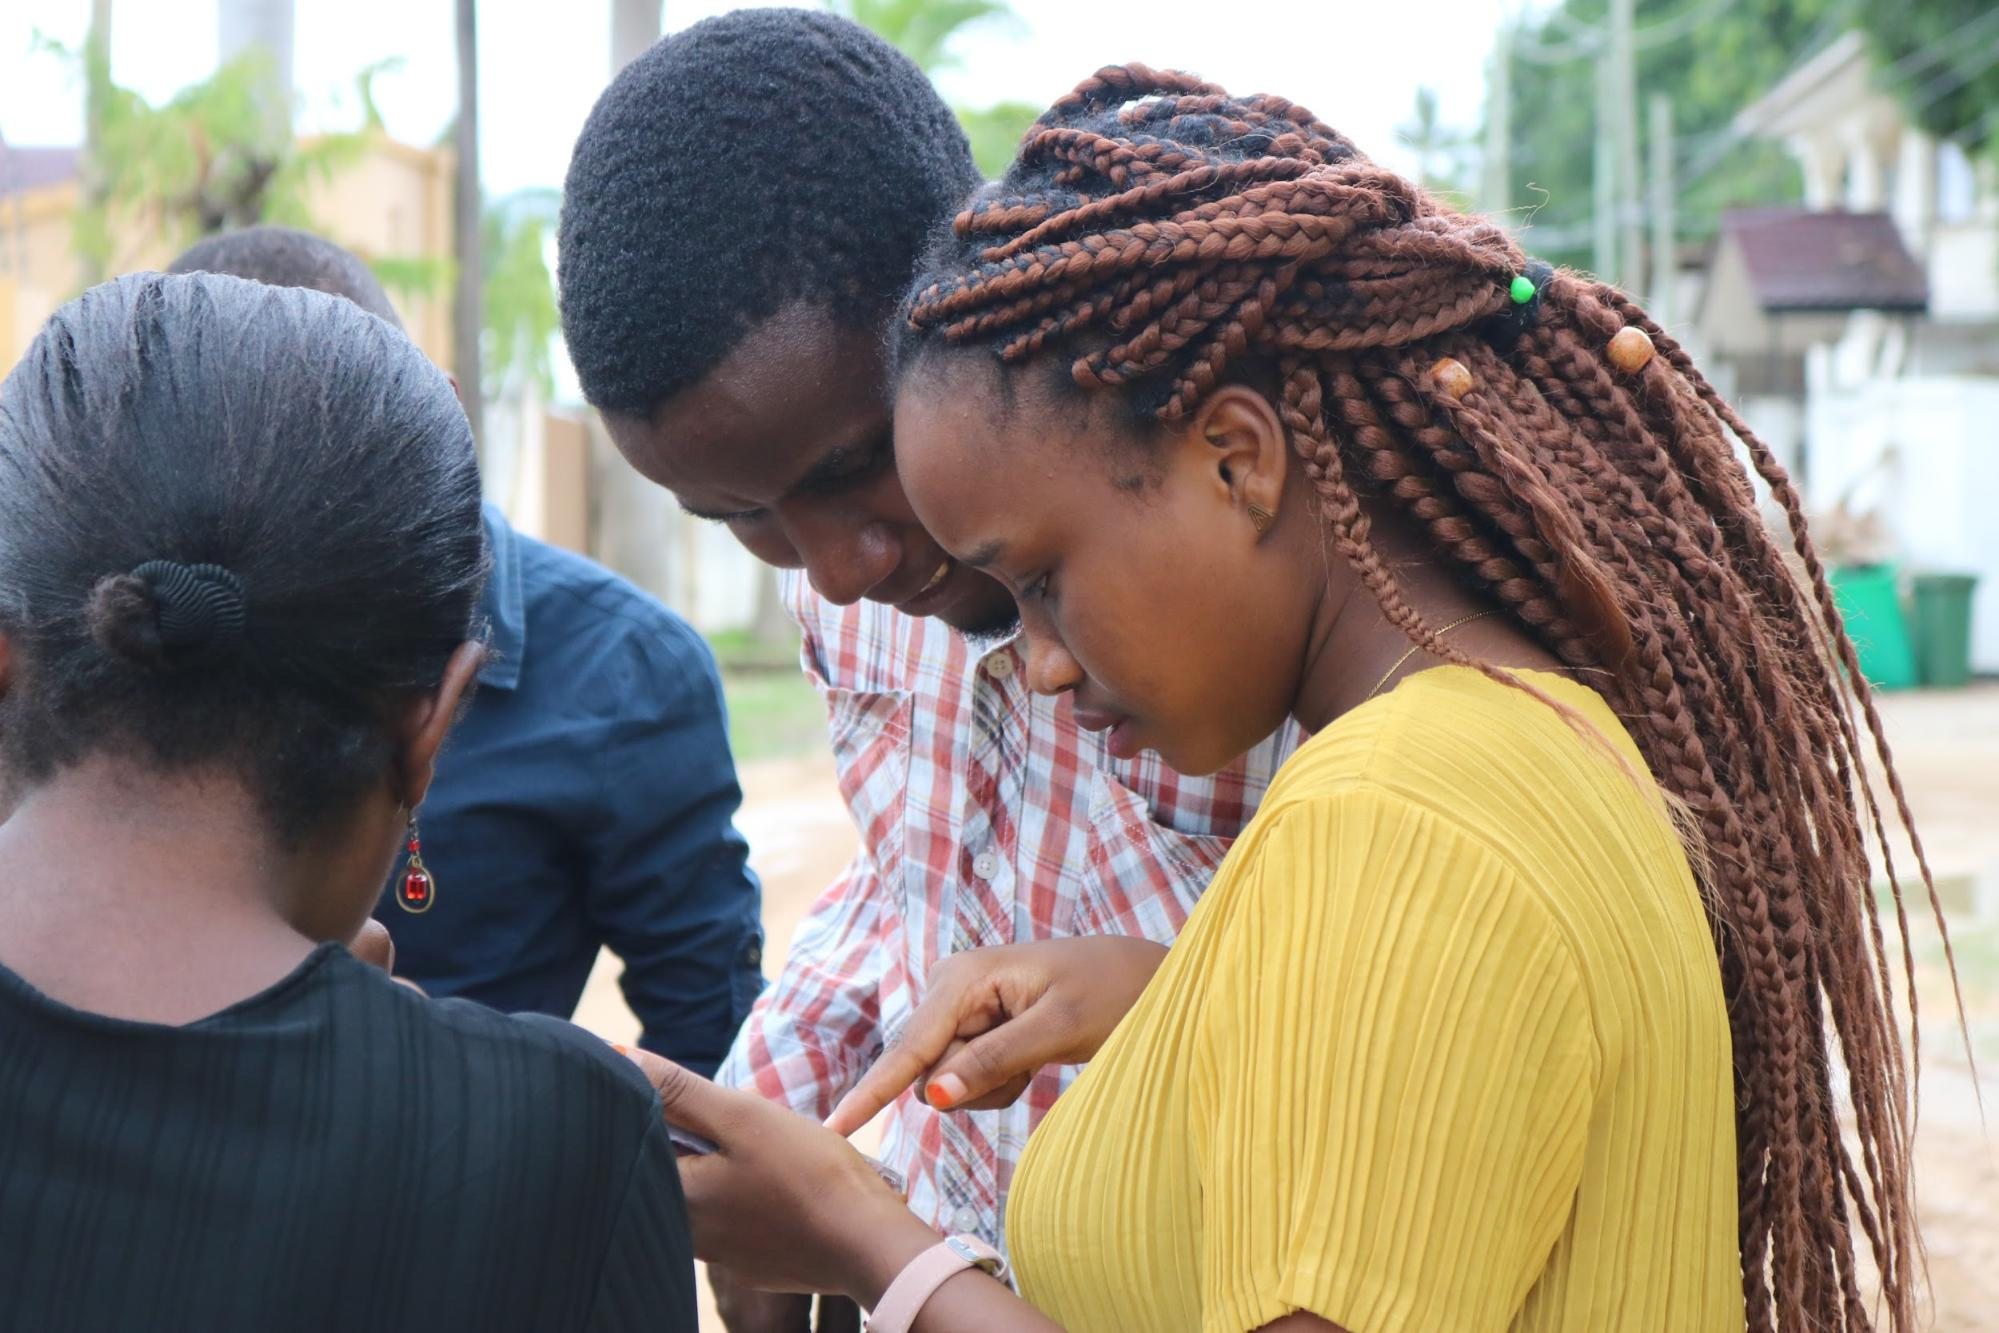
\includegraphics[width=0.8\textwidth]{images/image16.jpg}
        \caption{Practical ODK Training at the OMDTZ Office}
    \end{figure}

\subsection{QGIS Training}

    The team covered an overview of QGIS and how to add different data layers such as vector, raster and delimited text layers i.e. Comma Separated Value (CSV). We focused on this since the project involved the use of these file formats. The training also covered how to clean data using QGIS. Nipe Fagio staff were trained on different tools of OpenStreetMap and how they can use them in their work.

\subsection{Creation of Kobo Toolbox  server for data aggregation}

    KoBo Toolbox is a tool for mobile data collection that allows data collection using mobile devices such as smartphones or tablets, as well as paper or computers. During training, OMDTZ and Nipefagio created and configured a Kobo Toolbox server which will be used for the zero waste project implemented  by Nipe Fagio
    
    The server created will help Nipe Fagio to manage data collection easily through an online user interface, managing data quality by monitoring the data after collection and download it for advanced analysis in different formats such as Excel (XLS, CSV), KML and other formats supported by QGIS.
    
    The server is cost effective, quick and reliable and allows enormous data collection using mobile phone applications powered by Android. It also supports online and offline data collection. The server developed for Nipe Fagio can be accessed \href{https://kf.nipefagio.org/accounts/login/?next=/#/}{here}\footnote{https://kf.nipefagio.org/accounts/login/?next=/#/ (KoboToolBox login required)} (KoboToolBox login required). 
	
\subsection{Data Collection Tools}

    After the training on how to use the ODK application and creation of Kobo Toolbox server was done, a detailed assessment of the household questionnaires for Zero Waste using KoBo Toolbox and excel sheets integrated with ODK was covered. The questionnaire/form created focusing on Zero/No Waste in Dar es Salaam as requested by Nipe Fagio can be found \href{https://docs.google.com/spreadsheets/u/4/d/1TPp0CnafbNPQsICsMcPt7qCr5c4rztRn4qOA7dv2TpA/edit?usp=sharing}{here}\footnote{https://docs.google.com/spreadsheets/u/4/d/1TPp0CnafbNPQsICsMcPt7qCr5c4rztRn4qOA7dv2TpA/edit?usp=sharing}. 
    
    The form was well designed to allow Nipe Fagio volunteers and staff to get as much detail/information as possible in order to avoid time-consuming. The volunteers then went out to the Regent Estate subward to collect  data on Zero Waste using ODK and OMK application for navigation. 

\subsection{Map Literacy}

    During the training, a session of map reading was conducted to ensure all participants are able to read  maps. Two versions of maps were available; one with OSM ]data and the other with an aerial imagery background.
    
    To get started, participants were asked to identify known points/landmarks that they recognize on the map, and supported until they could do so. Participants were able to locate different features on a map, although in some cases not to the exact building/feature but closer. They were also able to update some street names that were missing on the printed map and new administrative boundaries such as Kiembe Samaki subward which was formerly located between Barabara ya Mwinyi and Kilakala subwards. 


\subsection{Preparation of Building Clustering and Non-clustering Randomization Manuals}

    As part of sharing technical skills , OMDTZ prepared manuals for Nipe Fagio so as to pass through during the execution of the project. Building randomization manual equipped them with skills to make random sampling of buildings for household survey.
    
    In order to obtain buildings in QGIS using clustering and randomization methodology as part of scientific research sampling, different tools are required such as a computer preinstalled with QGIS software and QuickOSM plugin installed, vector data i.e. the boundary of the coverage area, and/or satellite imagery.

\subsection{Waste Management Pilot in Mapped Areas With Nipe Fagio}

    Waste management pilot involved mapping and validating trash data that had been digitized using the river mapping drone imagery.
    
    \begin{figure} %[H] 
        \centering
        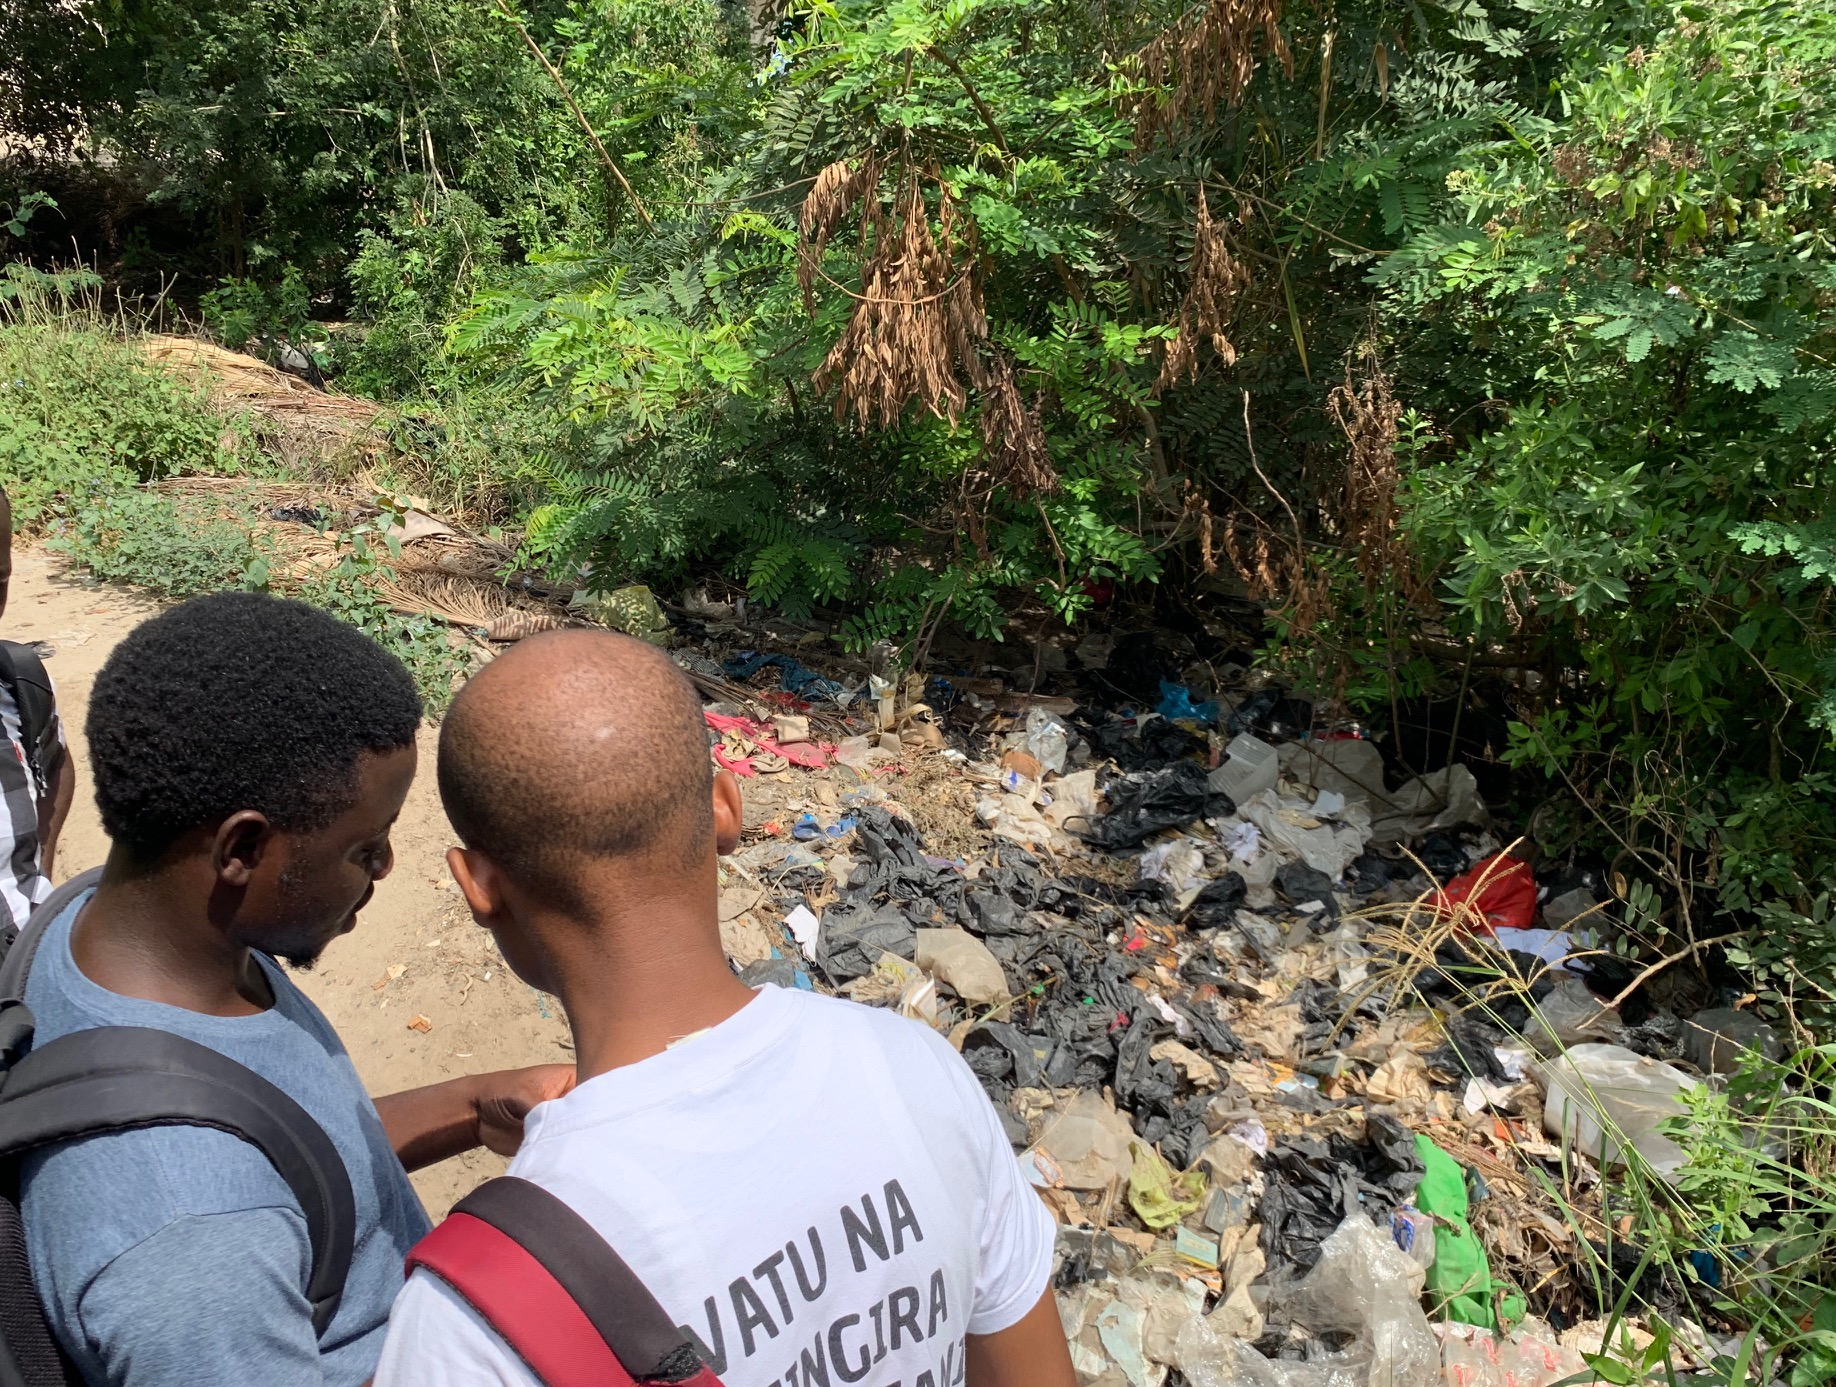
\includegraphics[width=0.8\textwidth]{images/image5.jpg}
        \caption{Nipe Fagio team validating trash Pile along Kibangu river}
    \end{figure}

\subsection{Questionnaire}

    This method involved open and close ended questions which were used to collect data or information from the field within Kimara Stop Over subward along Gide and Kibangu rivers.

    OMDTZ and Nipefagio teams filled the information using observation method of data collection. This method implies the collection of information by one’s own observation i.e. without interviewing the community. From this method information obtained relates to what is currently happening on the river.
    
    \begin{figure} %[H] 
        \centering
        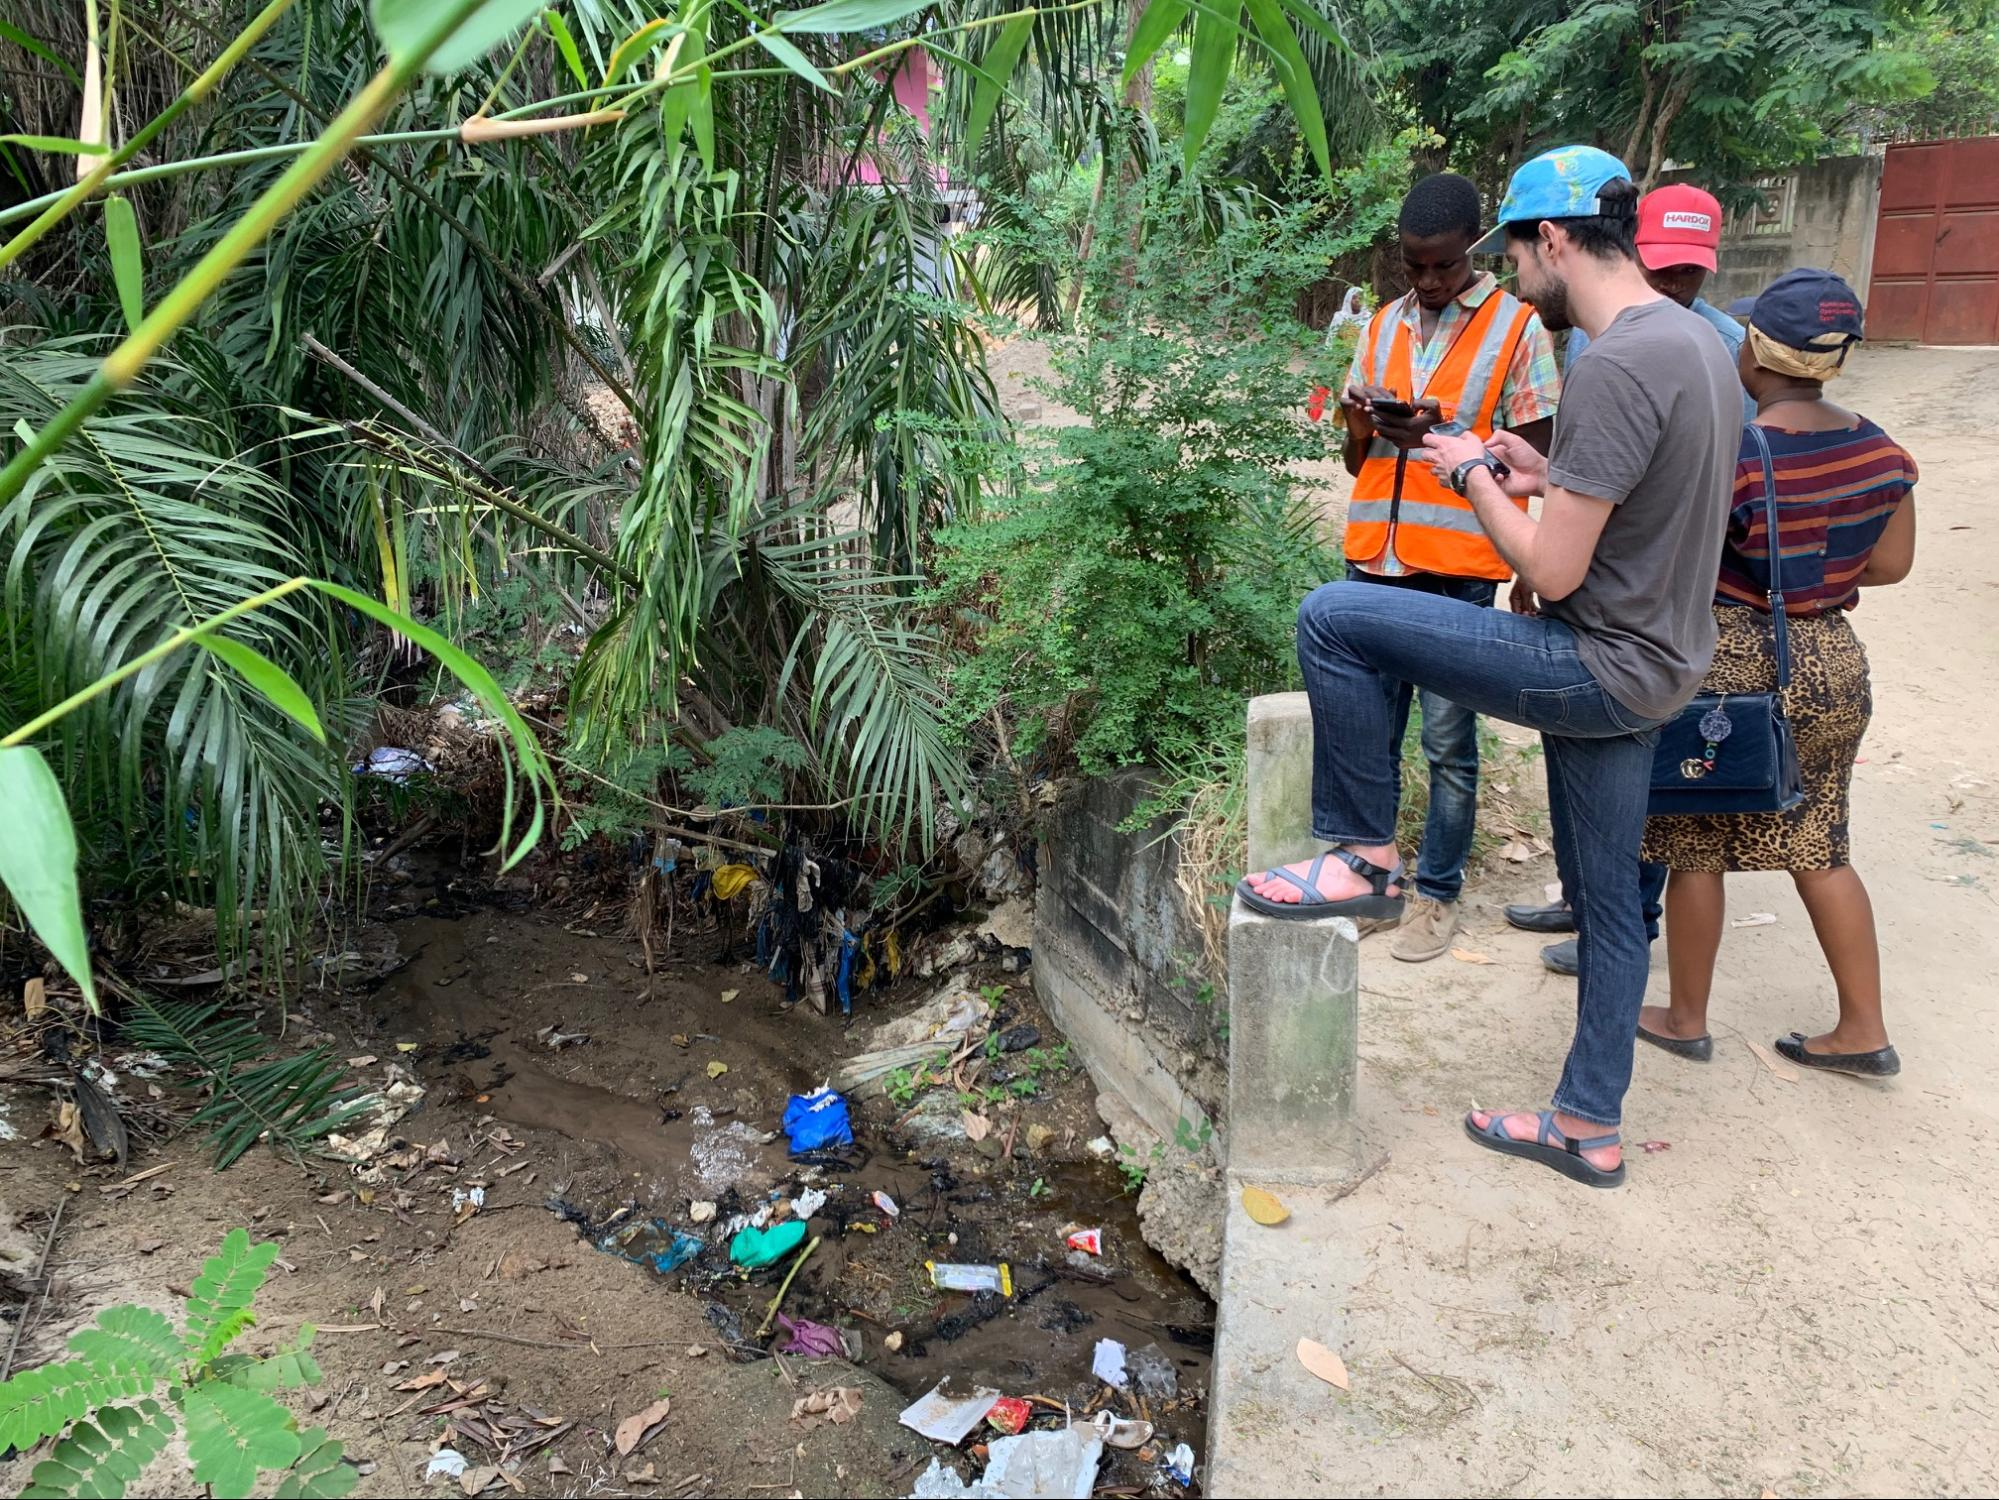
\includegraphics[width=0.8\textwidth]{images/image8.jpg}
        \caption{Recording undigitized trash pile along a tributary of Gide river, Kimara Stop Over}
    \end{figure}

\subsection{Data Cleaning using OpenRefine}

    \href{http://openrefine.org/}{OpenRefine}\footnote{http://openrefine.org/} is an open source software formerly known as Google Refine━is a powerful tool for working with messy data, cleaning it, transforming it from one format into another, and extending it with web services and external data.

    The OMDTZ team conducted a training on data cleaning using sample data from the "People Win River Win" project,  we firstly installed OpenRefine to their computers i.e. 3 Nipe Fagio staff followed by intensive OpenRefine training. 
\subsection{Preparation of Interactive Web Map}

    The OMDTZ team also conducted a simple but effective training to 3 Nipe Fagio staff on data visualization using \href{http://umap.openstreetmap.fr/en/}{uMap}\footnote{http://umap.openstreetmap.fr/en/}  as one of the  web based platforms used to visualize and share data openly and interactively.

\section{Activity 4: Routing}

\subsection{Overview}
    After the collection of drone data and analysis of solid waste sites was complete, the final deliverable of this project was to create a routing scheme giving travel from various points in the city of Dar Es Salaam to the Pugu Hills Dump site in _________.  This routing scheme could potentially be use

\subsection{Tools and Techniques Used}
    While many companies and mapping platforms have their own routing schemes (like Google or Bing), this exercise used only open data and open-source tools to create the routing model. The following tools and data sources were used in the creation of this schema:
    
    \begin{itemize}
        \item \textbf{PostgreSQL}
        A free and open-source relational database system used to host and manipulate the vector data collected during this project using the Structure Query Language (SQL).
        \item \textbf{PostGIS}
        An extension to PostgreSQL required for storing and manipulating spatial data.  
        \item \textbf{QGIS}
        An open-source Geographic Information System used as the graphic shell for our PostGIS work
        \item \textbf{PostGIS}
        \item \textbf{PostGIS}
    \end{itemize}

\subsubsection{PostgreSQL and PGRouting}

\subsubsection{Integrating Solid Waste Data with Routing Schema}

\subsection{Results}

\section{Conclusion}

    \begin{multicols}{2}
    \lipsum[0-5]
    \end{multicols}

\subsection{Achievements}

    \begin{multicols}{2}
    \lipsum[0-5]
    \end{multicols}

\subsection{Challenges}

    \begin{multicols}{2}
    \lipsum[0-5]
    \end{multicols}

\subsection{Lessons Learned}

    \begin{multicols}{2}
    \lipsum[0-5]
    \end{multicols}
    
\subsection{Recommendations}

    \begin{multicols}{2}
    \lipsum[0-5]
    \end{multicols}

\section{Acknowledgements}

    \begin{multicols}{2}
    \lipsum[0-5]
    \end{multicols}

\section{References}

    \begin{multicols}{2}
    \lipsum[0-5]
    \end{multicols}

\end{document}

